\documentclass{beamer}
\usepackage{listings}
\usepackage{graphicx}
\usepackage{bm}
\usepackage{amsmath,amssymb,xcolor,graphicx,url,natbib}
\usepackage{amsthm}
\usepackage{subfigure} % allow matrices of figures
\bibliographystyle{abbrv}

\newcommand{\bd}{\begin{description}} 
\newcommand{\ed}{\end{description}} 
\newcommand{\bi}{\begin{itemize}} 
\newcommand{\ei}{\end{itemize}} 

%\logo{
\includegraphics[width=2cm]{plots/TAB_col_white_background.eps}}

\addtobeamertemplate{frametitle}{}{
	\vspace{-0.6cm}\hfill\raisebox{-0.65ex}{
\includegraphics[height=1cm]{plots/TAB_col_white_background.eps}}}

\setbeamertemplate{footline}{\scriptsize
	\hfill \insertframenumber
}


\title{\fontsize{14pt}{12pt}\selectfont Dynamics of Elastic Particles in Viscous Shear Flow}
%\subtitle{}
\author{
	Hao Ye \\ \textit{Department of Mathematics} \\
	\vspace{0.5cm} 
	Supervisors: \\Matthias Heil, Draga Pihler-Puzović
}
%\date{\tiny Please update course code, project number, name and Student ID!}
\begin{document}

\begin{frame}[plain] 
	\maketitle 
	
	%\vfill 
	
	\begin{center}
		
\includegraphics[height=1.2cm]{plots/TAB_col_white_background.eps} 
	\end{center}
\end{frame}

%%%%%%%%%%%%%%%%%%%%%%%%%%%%%%%%%%%%%%%%%%%%%%%%%%%%%%%%%%%%%%%%%%%%%%

%\frame{\titlepage}

%%%%%%%%%%%%%%%%%%%%%%%%%%%%%%%%%%%%%%%%%%%%%%%%%%%%%%%%%%%%%%%%%%%%%%

\begin{frame}
	\frametitle{Applications: particles in shear flow}
	\begin{overlayarea}{\textwidth}{\textheight}
		\vspace{-0.2cm}
    	\begin{figure}
			\begin{minipage}{0.4\linewidth}
				\centering
				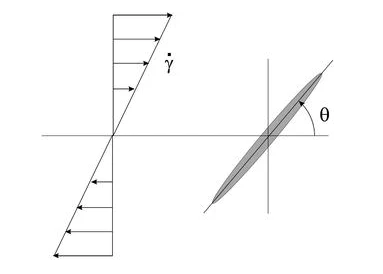
\includegraphics[width=\linewidth]{plots/application2.png} 
			 \centering \scriptsize A rigid ellipsoid \cite{yasuda2004experimental}.
			\end{minipage}
		\begin{minipage}{0.5\linewidth}
			\centering
			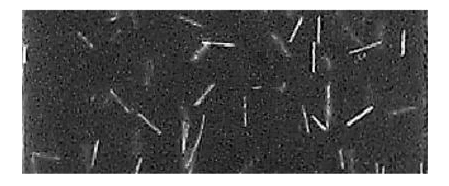
\includegraphics[width=\linewidth]{plots/application2_2.png} 
			\centering \scriptsize Vinylon fibers (paper industry) \cite{yasuda2004experimental}.
		\end{minipage}\vspace{0.5cm}
	\begin{minipage}{0.3\linewidth}
		\centering
		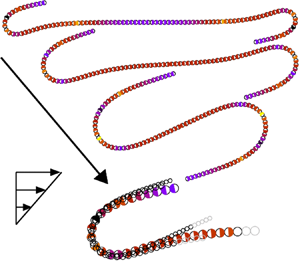
\includegraphics[width=\linewidth]{plots/application6.png} 
		\centering \scriptsize Elongated elastic fibres \cite{zuk2021universal}.
	\end{minipage}
		\begin{minipage}{0.32\linewidth}
		\centering
		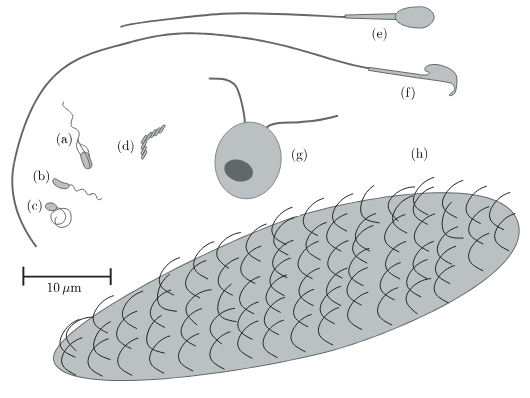
\includegraphics[width=\linewidth]{plots/application1.png} 
		\centering \scriptsize Sketches of microscopic swimmers, to scale \cite{lauga2009hydrodynamics}.
	\end{minipage}
		\begin{minipage}{0.35\linewidth}
	\centering
	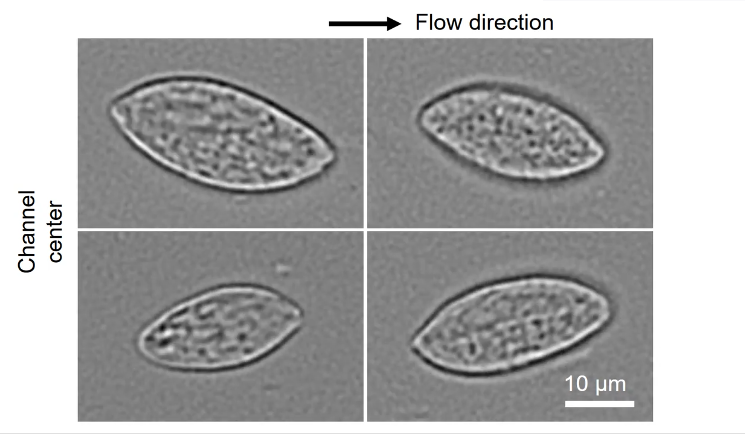
\includegraphics[width=\linewidth]{plots/application5.png}
	\centering \scriptsize Tank-treading motion of cells (video) \cite{gerum2022viscoelastic}.
\end{minipage}
		\end{figure}
	\end{overlayarea}
\end{frame}

%%%%%%%%%%%%%%%%%%%%%%%%%%%%%%%%%%%%%%%%%%%%%%%%%%%%%%%%%%%%%%%%%%%%%%

\begin{frame}
	\frametitle{Introduction: Jeffery orbits}
	\begin{overlayarea}{\textwidth}{\textheight}
		\vspace{-0.2cm}
	\begin{columns}
	\column{.6\textwidth}
	\begin{figure}[htb]
		\begin{center}
			% specify width as 80% of the width of the text on the page
			% we can also specify a width in centimetres, e.g. [width=8cm]
			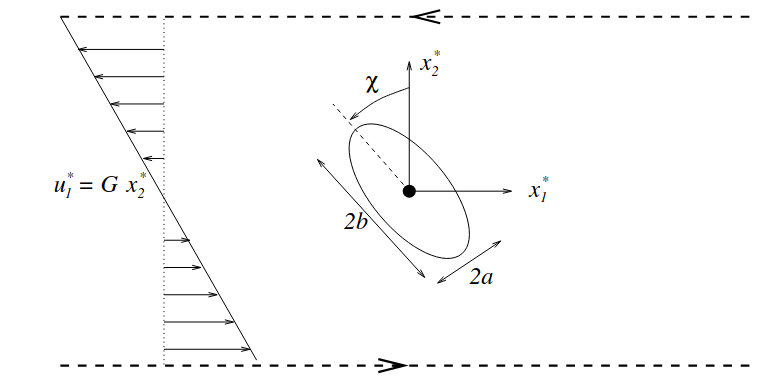
\includegraphics[width=1\textwidth]{plots/jeffery.png}
		\end{center}
		%	\setlength{\abovecaptionskip}{-0.5 cm}
	\end{figure}
	\column{.55\textwidth}
	\small
	\bi
	\item In 1922, Jeffery published his seminal work on the periodic tumbling motion of rigid ellipsoidal particles in shear flow.
	\item This motion is parameterized only by the initial orientation.
	\ei 
\end{columns}
\vspace{0.5cm}
\bi
\item If vorticity $\omega\neq 0$, particles will undergo a parodic rotation (Jeffery orbits).
	\item The orbital period is dependent on the aspect ratio of the particle (shape!).
\item However, do they always rotate periodically (for other shapes)?
\ei
		%\vspace{0.1cm}
	\end{overlayarea}
\end{frame}

%%%%%%%%%%%%%%%%%%%%%%%%%%%%%%%%%%%%%%%%%%%%%%%%%%%%%%%%%%%%%%%%%%%%%%


\begin{frame}
	\frametitle{Introduction: boomerang-shaped particles}
	\begin{overlayarea}{\textwidth}{\textheight}
		\vspace{-0.5cm}
		\begin{columns}
		\column{.55\textwidth}
		\begin{figure}[htb]
			\begin{center}
				% specify width as 80% of the width of the text on the page
				% we can also specify a width in centimetres, e.g. [width=8cm]
				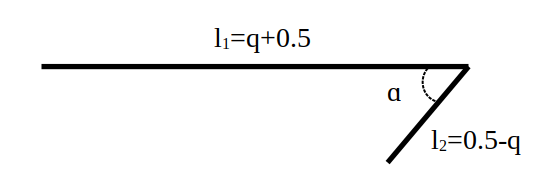
\includegraphics[width=0.8\textwidth]{plots/geometry2.png}
			\end{center}
			%	\setlength{\abovecaptionskip}{-0.5 cm}
		\end{figure}
		\column{.6\textwidth}
		\small
		\bi
		\item $q \in [0,0.5), \alpha \in (0,2\pi)$.
		\item Extreme cases:
		$
			\label{eqn:1}
			\left.
			\begin{aligned}
				&\alpha=0,\pi \\
				&	q=0.5
			\end{aligned}
			\right\}\Longrightarrow \text{straight rod},$ 
			
			$q=0, \alpha \neq 0, \pi \Longrightarrow \text{same arm length}.
		$
		\ei 
	\end{columns}
\vspace{0.1cm} \small
\bi
\item As $q$ increases, the short arm shortens while the long arm lengthens.
\ei \vspace{-0.15cm}
	\begin{columns}
	\column{.55\textwidth}
	Results\footnote{\tiny Roggeveen J V, Stone H A. Motion of asymmetric bodies in two-dimensional shear flow[J]. Journal of Fluid Mechanics, 2022, 939: A23.}:
\bi
\item White: periodic cross-streamline motion while tumbling. \item Grey: persistent cross-streamline drift at a fixed angle (asymmetric, small $\alpha$). \textbf{Do not rotate!}
\ei 
\column{.5\textwidth}
	\begin{figure}[htb]
	\begin{center}
		% specify width as 80% of the width of the text on the page
		% we can also specify a width in centimetres, e.g. [width=8cm]
		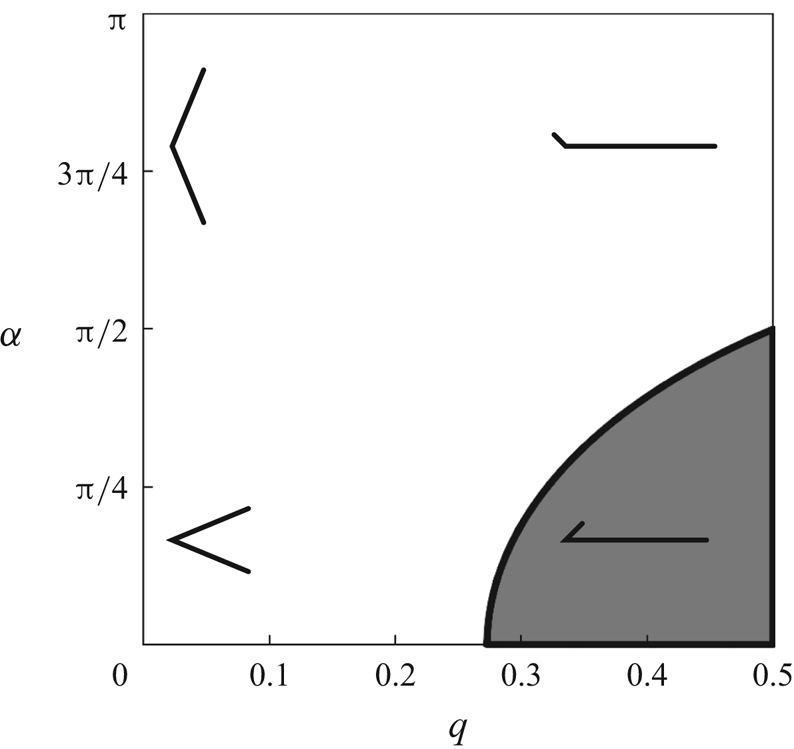
\includegraphics[width=0.85\textwidth]{plots/stone.png}
	\end{center}
	%	\setlength{\abovecaptionskip}{-0.5 cm}
\end{figure}
	\end{columns}
	\end{overlayarea}
\end{frame}

%%%%%%%%%%%%%%%%%%%%%%%%%%%%%%%%%%%%%%%%%%%%%%%%%%%%%%%%%%%%%%%%%%%%%%





\begin{frame}
	\frametitle{Introduction: boomerang-shaped particles}
	\begin{overlayarea}{\textwidth}{\textheight}
		\vspace{-0.3cm}
		\begin{columns}
			\column{.55\textwidth}
			\begin{figure}[htb]
				\begin{center}
					% specify width as 80% of the width of the text on the page
					% we can also specify a width in centimetres, e.g. [width=8cm]
					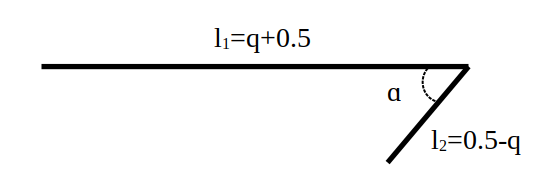
\includegraphics[width=0.8\textwidth]{plots/geometry2.png}
				\end{center}
				%	\setlength{\abovecaptionskip}{-0.5 cm}
			\end{figure}
			\column{.6\textwidth}
			\small
			\bi
			\item $q \in [0,0.5), \alpha \in (0,2\pi)$.
			\item Extreme cases:
			$
			\label{eqn:1}
			\left.
			\begin{aligned}
				&\alpha=0,\pi \\
				&	q=0.5
			\end{aligned}
			\right\}\Longrightarrow \text{straight rod},$ 
			
			$q=0, \alpha \neq 0, \pi \Longrightarrow \text{same arm length}.
			$
			\ei 
		\end{columns}
		\vspace{0.1cm} \small
		\bi
		\item As $q$ increases, the short arm shortens while the long arm lengthens.
		\ei \vspace{0.1cm}
		\begin{columns}
			\column{.55\textwidth}
			Results\footnote{\tiny Roggeveen J V, Stone H A. Motion of asymmetric bodies in two-dimensional shear flow[J]. Journal of Fluid Mechanics, 2022, 939: A23.}:
			\bi
			\item Of these four fixed orientations, two differ from the other two by an angle of $\pi$ but possess the same shapes.
			\ei \vspace{0.2cm}
			\column{.6\textwidth}
			\vspace{-0.5cm}
			\begin{figure}[htb]
				\begin{center}
					% specify width as 80% of the width of the text on the page
					% we can also specify a width in centimetres, e.g. [width=8cm]
					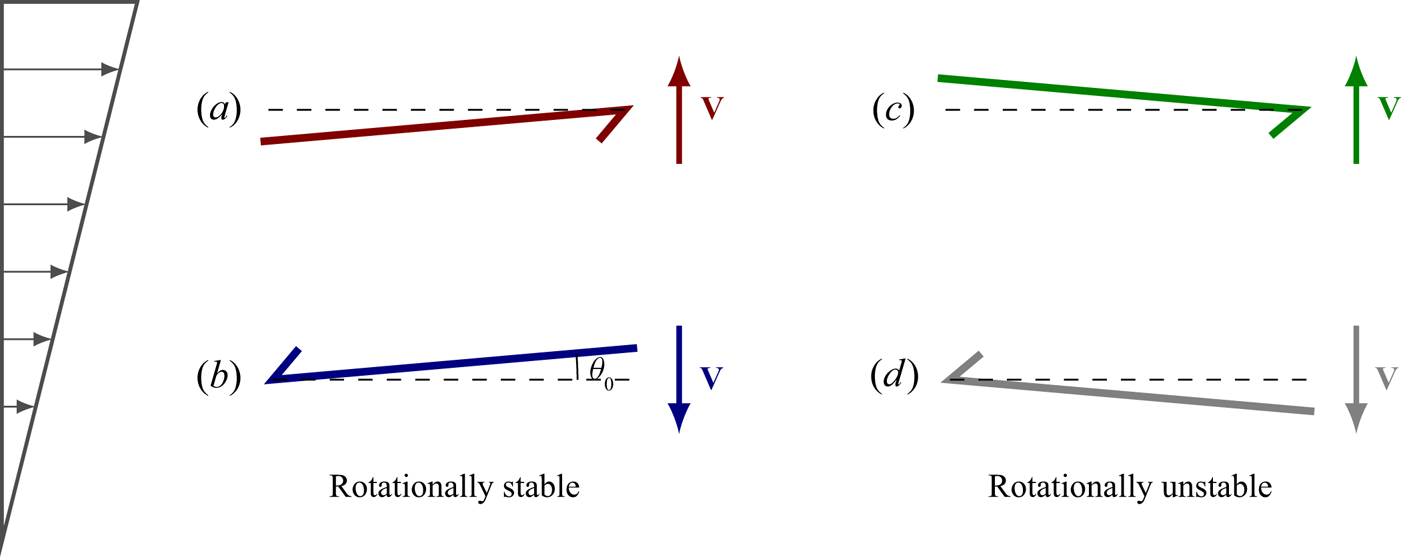
\includegraphics[width=0.9\textwidth]{plots/stone3.png}
				\end{center}
				%	\setlength{\abovecaptionskip}{-0.5 cm}
			\end{figure}
		\end{columns}
	\end{overlayarea}
\end{frame}

%%%%%%%%%%%%%%%%%%%%%%%%%%%%%%%%%%%%%%%%%%%%%%%%%%%%%%%%%%%%%%%%%%%%%%


\begin{frame}
	\frametitle{Frames}
	\begin{overlayarea}{\textwidth}{\textheight}
	%\vspace{0.3cm}	
\begin{itemize}
	\item  Particle-fixed reference frame $\{\mathbf{e_1},\mathbf{e_2},\mathbf{e_3}\}$.
	\item Laboratory reference frame $\{\mathbf{e'_1},\mathbf{e'_2},\mathbf{e'_3}\}$.
	\item Bridge linking the two frames, showing the orientation $\theta(t)$ (small proof).
	\item Initially, the particle-fixed reference frame is attached to the laboratory reference frame such that $\mathbf{e'_3}=\mathbf{e_3}$. \\\vspace{0.3cm}But does this condition $\mathbf{e'_3}=\mathbf{e_3}$ hold all the time?
	\begin{figure}[htb]
		\begin{center}
			% specify width as 80% of the width of the text on the page
			% we can also specify a width in centimetres, e.g. [width=8cm]
			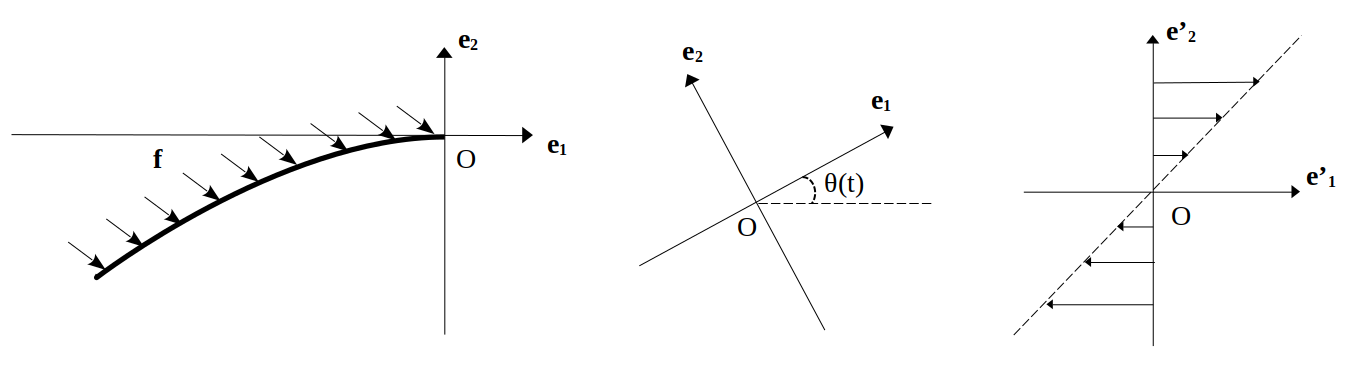
\includegraphics[width=0.9\textwidth]{plots/frames_general.png}
		\end{center}
		%	\setlength{\abovecaptionskip}{-0.5 cm}
	\end{figure}
	%\selectfont \fontsize{10}{15}\selectfont
\end{itemize}
	\end{overlayarea}
\end{frame}

%%%%%%%%%%%%%%%%%%%%%%%%%%%%%%%%%%%%%%%%%%%%%%%%%%%%%%%%%%%%%%%%%%%%%%

\begin{frame}
	\frametitle{Small proof}
	\begin{overlayarea}{\textwidth}{\textheight}
		\vspace{-0.3cm}	
\begin{figure}[htb]
	\begin{center}
		% specify width as 80% of the width of the text on the page
		% we can also specify a width in centimetres, e.g. [width=8cm]
		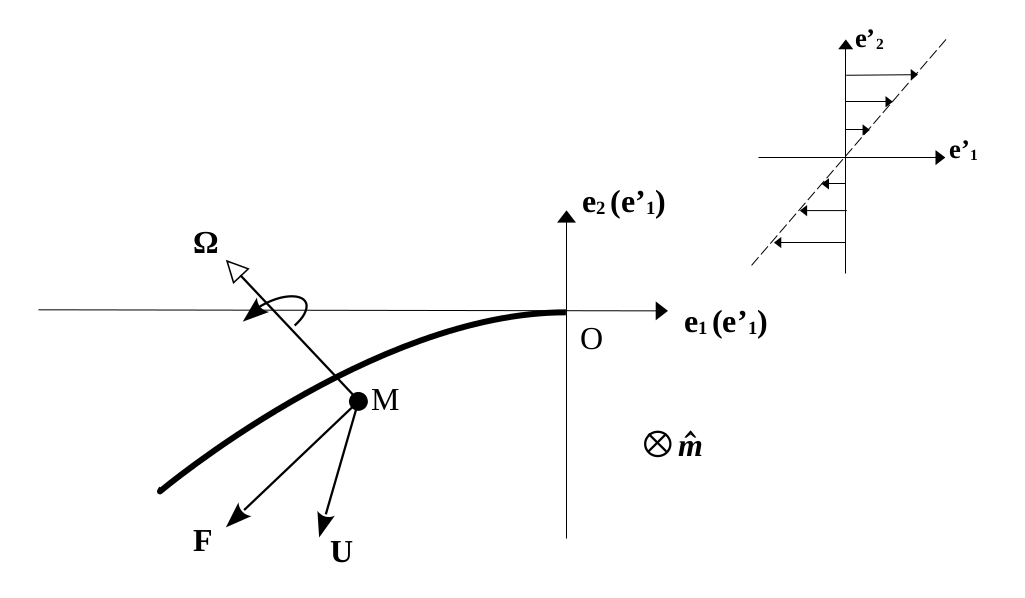
\includegraphics[width=0.7\textwidth]{plots/relection_general.png}
	\end{center}
	%	\setlength{\abovecaptionskip}{-0.5 cm}
\end{figure}
\begin{equation*}
	\text{Reflection:}\quad \mathbf{U}\mapsto(\mathbf{I}-2\,\mathbf{\hat{m}}\mathbf{\hat{m}})\cdot\mathbf{U},\quad 	\bm{\Omega}\mapsto-(\mathbf{I}-2\mathbf{\hat{m}}\mathbf{\hat{m}})\cdot\bm{\Omega}.
\end{equation*}
\begin{equation*}
	\text{Uniqueness:}\quad(\mathbf{I}-2\,\mathbf{\hat{m}}\mathbf{\hat{m}})\cdot\mathbf{U}=\mathbf{U}, \quad 	-(\mathbf{I}-2\,\mathbf{\hat{m}}\mathbf{\hat{m}})\cdot\bm{\Omega}=\bm{\Omega}.
\end{equation*}
\begin{equation*}
	\mathbf{U}\cdot\mathbf{\hat{m}}=0, \quad \bm{\Omega}\varpropto\mathbf{\hat{m}}.
\end{equation*}
\vspace{-0.5cm}	
\bi
\item $\mathbf{e'_3}=\mathbf{e_3}$ holds permanently rather than only initially.
%\selectfont \fontsize{10}{15}\selectfont
\ei
	\end{overlayarea}
\end{frame}

%%%%%%%%%%%%%%%%%%%%%%%%%%%%%%%%%%%%%%%%%%%%%%%%%%%%%%%%%%%%%%%%%%%%%%


\begin{frame}
	\frametitle{Small proof}
	\begin{overlayarea}{\textwidth}{\textheight}
		\vspace{-0.3cm}	
		\begin{figure}[htb]
			\begin{center}
				% specify width as 80% of the width of the text on the page
				% we can also specify a width in centimetres, e.g. [width=8cm]
				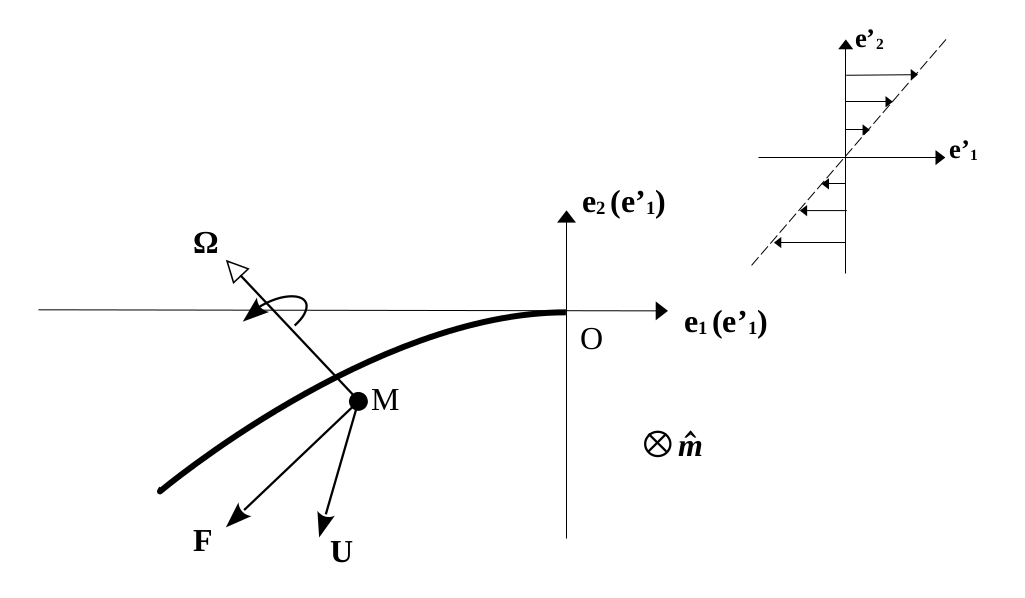
\includegraphics[width=0.45\textwidth]{plots/relection_general.png}
			\end{center}
			%	\setlength{\abovecaptionskip}{-0.5 cm}
		\end{figure}
	\vspace{-0.3cm}
		\begin{figure}[htb]
		\begin{center}
			% specify width as 80% of the width of the text on the page
			% we can also specify a width in centimetres, e.g. [width=8cm]
			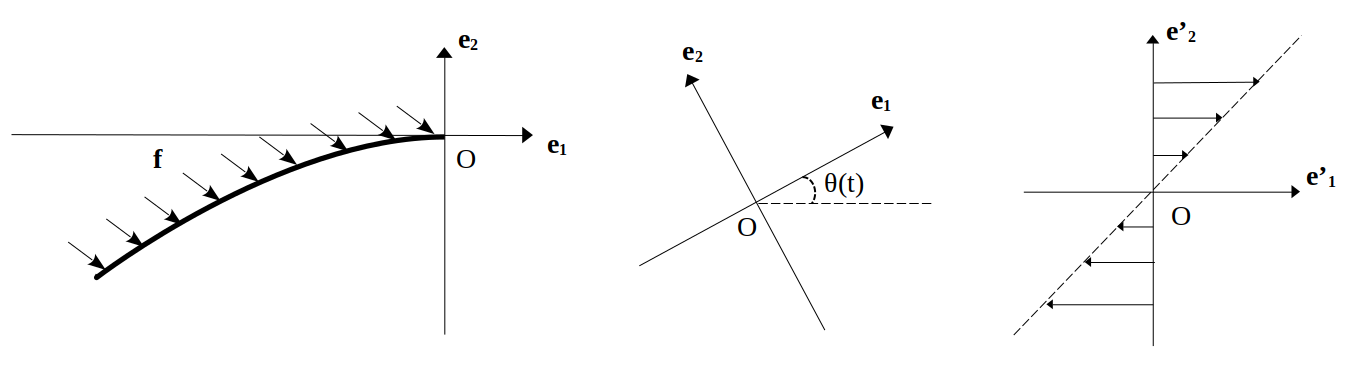
\includegraphics[width=0.7\textwidth]{plots/frames_general.png}
		\end{center}
		%	\setlength{\abovecaptionskip}{-0.5 cm}
	\end{figure}
		\bi
		\item $\mathbf{e'_3}=\mathbf{e_3}$ holds permanently rather than only initially.
		\item Bridge linking the two frames, showing a single variable $\theta(t)$ (it is enough!).
		%\selectfont \fontsize{10}{15}\selectfont
		\ei
	\end{overlayarea}
\end{frame}

%%%%%%%%%%%%%%%%%%%%%%%%%%%%%%%%%%%%%%%%%%%%%%%%%%%%%%%%%%%%%%%%%%%%%%

\begin{frame}
	\frametitle{Fluid mechanics}
	\begin{overlayarea}{\textwidth}{\textheight}
		%\vspace{-0.3cm}
		\begin{columns}
			\column{.55\textwidth}	
		\begin{figure}[htb]
			\begin{center}
				% specify width as 80% of the width of the text on the page
				% we can also specify a width in centimetres, e.g. [width=8cm]
				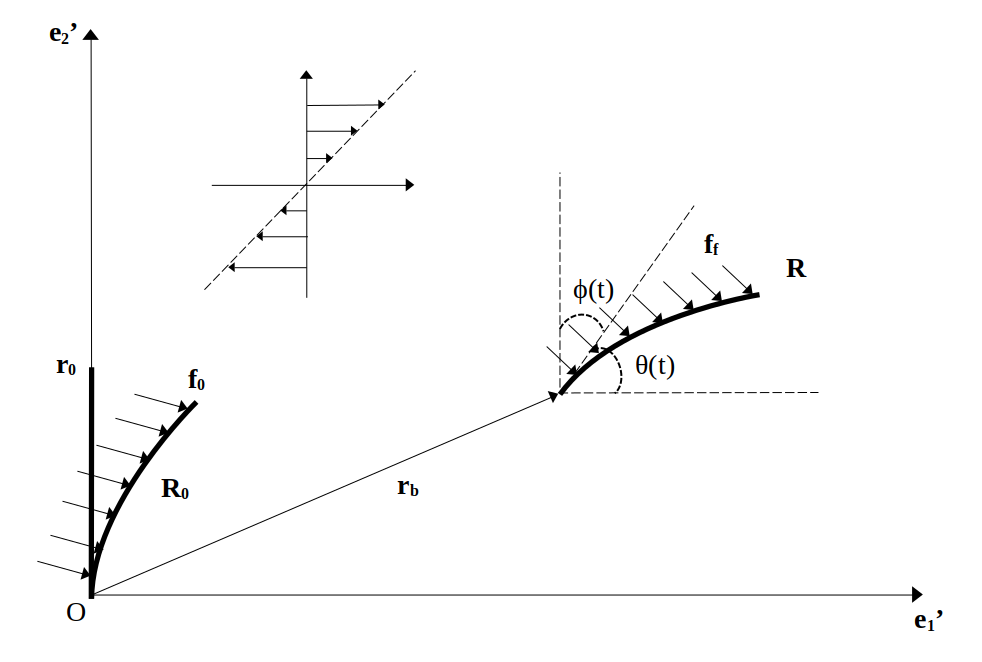
\includegraphics[width=1\textwidth]{plots/r0.png}
			\end{center}
			%	\setlength{\abovecaptionskip}{-0.5 cm}
		\end{figure}
		Dimensional variables (asterisks): 
		
		undeformed: $\mathbf{r}_0^*(\xi^*)=(0,\xi^*)^T, \quad  \xi^*\in [0,\mathcal{L}]$.
		
		deformed: $\mathbf{R}_0^*(t^*,\xi^*)$.	
		\column{.5\textwidth}
			\begin{equation*}
			\mathbf{R}^*(t^*,\xi^*)=\mathbf{\mathcal{R}}\,\mathbf{R}_0^*(t^*,\xi^*)+\mathbf{r}_b^*(t^*),
		\end{equation*}
		where $$\mathbf{\mathcal{R}}=\left(\begin{aligned}
				&\cos(\phi(t^*))\quad -\sin(\phi(t^*)) \\
				&\sin(\phi(t^*))\quad \cos(\phi(t^*))
			\end{aligned}\right).$$
		\normalsize \begin{equation*}
			\theta(t^*)=\frac{\pi}{2}-\phi(t^*).
		\end{equation*}
		\end{columns}
	\end{overlayarea}
\end{frame}

%%%%%%%%%%%%%%%%%%%%%%%%%%%%%%%%%%%%%%%%%%%%%%%%%%%%%%%%%%%%%%%%%%%%%%



\begin{frame}
	\frametitle{Fluid mechanics}
	\begin{overlayarea}{\textwidth}{\textheight}
		%\vspace{-0.3cm}	
	\begin{equation*}
		\mathbf{U}^{\infty*}(\mathbf{R}^*(t^*,\xi^*))=\dot{\gamma}\left(\mathbf{R}^*(t^*,\xi^*)\cdot\mathbf{e}_y\right)\cdot\mathbf{e}_x,
	\end{equation*}
	\begin{equation*}
		\mathbf{U}^*=\frac{\partial\mathbf{R}^*(t^*,\xi^*)}{\partial t^*}.
	\end{equation*}
	\begin{equation*}
		\mathbf{e}_t=\frac{1}{|\frac{\partial\mathbf{R}^*(t^*,\xi^*)}{\partial\xi^*}|}\frac{\partial\mathbf{R}^*(t^*,\xi^*)}{\partial\xi^*}.
	\end{equation*}
	From the slender body theory, the traction is obtained as flows:
	\begin{equation*}
		\label{eqn:24}
		\mathbf{f}^*=c_\perp\left(\mathbf{I}-\frac{1}{2}\mathbf{e}_t\mathbf{e}_t\right)\cdot(\mathbf{U}^{\infty*}-\mathbf{U}^*),
	\end{equation*}
	where $c_\perp=\frac{4\pi\mu}{\ln{\frac{1}{\epsilon}}}$ is the drag coefficient.
	\end{overlayarea}
\end{frame}

%%%%%%%%%%%%%%%%%%%%%%%%%%%%%%%%%%%%%%%%%%%%%%%%%%%%%%%%%%%%%%%%%%%%%%

\begin{frame}
	\frametitle{Fluid mechanics}
	\begin{overlayarea}{\textwidth}{\textheight}
We non-dimensionalise the variables mentioned in this section using the following basic relationships:
\begin{equation*}
	\xi^*=\mathcal{L}\xi, \quad t^*=\frac{1}{\dot{\gamma}}\,t.
\end{equation*}
\vspace{-0.3cm}
Then, we have 
\begin{equation*}
	(\mathbf{r}_0^*, \mathbf{r}_b^*, \mathbf{R}_0^*, \mathbf{R}^*)^T=\mathcal{L}\cdot(\mathbf{r}_0, \mathbf{r}_b, \mathbf{R}_0, \mathbf{R})^T,
\end{equation*}
\begin{equation*}
	\mathbf{U}^{\infty*}=\mathcal{L}\dot{\gamma}\mathbf{U}^{\infty}, \quad \mathbf{U}^*=\mathcal{L}\dot{\gamma}\mathbf{U},
\end{equation*}
\begin{equation*}
	\mathbf{f}^*=c_\perp\,\mathcal{L}\,\dot{\gamma}\,\left(\mathbf{I}-\frac{1}{2}\mathbf{e}_t\mathbf{e}_t\right)\cdot(\mathbf{U}^{\infty}-\mathbf{U})=c_\perp\,\mathcal{L}\,\dot{\gamma}\,\mathbf{f}_{f},
\end{equation*}
where 
\begin{equation*}
	\mathbf{f}_f=\left(\mathbf{I}-\frac{1}{2}\mathbf{e}_t\mathbf{e}_t\right)\cdot(\mathbf{U}^{\infty}-\mathbf{U}),
\end{equation*}
is the non-dimensional fluid traction.
	\end{overlayarea}
\end{frame}

%%%%%%%%%%%%%%%%%%%%%%%%%%%%%%%%%%%%%%%%%%%%%%%%%%%%%%%%%%%%%%%%%%%%%%


\begin{frame}
	\frametitle{Solid Mechanics}
	\begin{overlayarea}{\textwidth}{\textheight}
		Non-dimensional equation by scaling the stresses
		and the applied traction on the beam’s effective Young’s modulus
	\begin{equation*}
		\label{eqn:29}
		E_{eff}=\frac{E}{(1-v^2)}. \quad \text{Then,}	\left(\begin{aligned}
			&\mathbf{f^*} \\
			&\mathbf{\sigma}_0^*
		\end{aligned}\right)
		=E_{eff}\left(\begin{aligned}
			&\textbf{f}_{s} \\
			&\mathbf{\sigma}_0
		\end{aligned}\right),
	\end{equation*}
where $\textbf{f}_{s}$ is the non-dimensional solid traction.
\vspace{0.35cm}
  
  The non-dimensional form of the principle of virtual displacements that governs the beam's deformation is given by (Kirchhoff-Love beam theory):
  \vspace{-0.2cm}
\begin{equation*}
	\begin{aligned}
		\int_0^1 \Bigg[ (\sigma_0 + \gamma) \delta \gamma 
		+ &\frac{1}{12} h^2 \kappa \delta \kappa \Bigg. \\
		&\Bigg. - \Bigg( \frac{1}{h} \sqrt{\frac{A}{a}}\, \textbf{f}_s - \Lambda^2 \frac{\partial^2 \textbf{R}_0}{\partial t^2} \Bigg) 
		\cdot \delta \textbf{R}_0 \Bigg] \sqrt{a}\, d\xi = 0.
	\end{aligned}
\end{equation*}
	\end{overlayarea}
\end{frame}

%%%%%%%%%%%%%%%%%%%%%%%%%%%%%%%%%%%%%%%%%%%%%%%%%%%%%%%%%%%%%%%%%%%%%%



\begin{frame}
	\frametitle{Solid Mechanics}
	\begin{overlayarea}{\textwidth}{\textheight}
Since the elastic beam is initially clamped at the origin, the boundary conditions are
\begin{equation*}
	\label{eqn:58}
	\mathbf{R}_0(\xi=0)\cdot\mathbf{e}_x=0,\quad \mathbf{R}_0(\xi=0)\cdot\mathbf{e}_y=0,
\end{equation*}
\begin{equation*}
	\label{eqn:60}
	\frac{d\left(\mathbf{R}_0(\xi=0)\cdot\mathbf{e}_x\right)}{d\xi}=0.
\end{equation*}
\vspace{-0.7cm}
\begin{figure}[htb]
	\begin{center}
		% specify width as 80% of the width of the text on the page
		% we can also specify a width in centimetres, e.g. [width=8cm]
		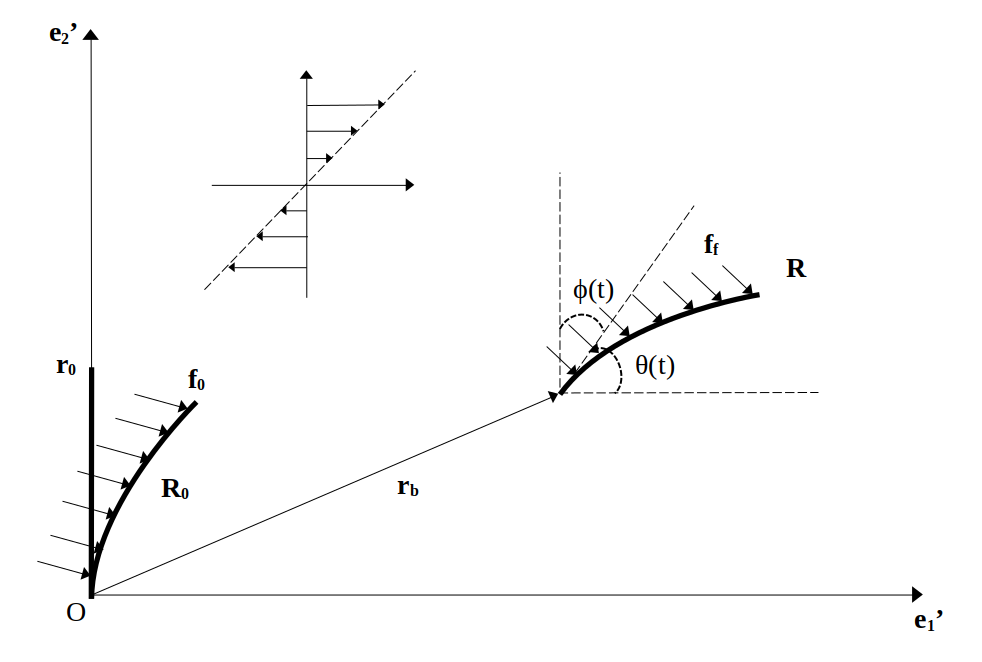
\includegraphics[width=0.7\textwidth]{plots/r0.png}
	\end{center}
	%	\setlength{\abovecaptionskip}{-0.5 cm}
\end{figure}
	\end{overlayarea}
\end{frame}

%%%%%%%%%%%%%%%%%%%%%%%%%%%%%%%%%%%%%%%%%%%%%%%%%%%%%%%%%%%%%%%%%%%%%%


\begin{frame}
	\frametitle{Fluid–solid coupling}
	\begin{overlayarea}{\textwidth}{\textheight}
Recall that
\begin{equation*}
	\label{eqn:102}
	\mathbf{f}^*=c_\perp\,\mathcal{L}\,\dot{\gamma}\,\mathbf{f}_{f}, \quad \mathbf{f}^*=E_{eff}\,\mathbf{f}_{s}.
\end{equation*}
Hence, the fluid applies traction to the beam, and the loading term in the solid equation are expressed by
\begin{equation*}
	\label{eqn:37}
	\textbf{f}_{s}=\frac{c_\perp\,\mathcal{L}\,\dot{\gamma}}{E_{eff}}\,\textbf{f}_{f}.
\end{equation*}
Then, we define the coefficient $\mathcal{I}$, which represents the coefficient of fluid-solid interaction and is expressed as:
\begin{equation*}
	\label{eqn:38}
	\mathcal{I}=\frac{c_\perp\,\mathcal{L}\,\dot{\gamma}}{E_{eff}}.
\end{equation*}
\tiny
Recall that
\begin{equation*}
		\int_0^1 \Bigg[ (\sigma_0 + \gamma) \delta \gamma 
		+ \frac{1}{12} h^2 \kappa \delta \kappa \Bigg. 
		\Bigg. - \Bigg( \frac{1}{h} \sqrt{\frac{A}{a}}\, \textbf{f}_s - \Lambda^2 \frac{\partial^2 \textbf{R}_0}{\partial t^2} \Bigg) 
		\cdot \delta \textbf{R}_0 \Bigg] \sqrt{a}\, d\xi = 0,
\end{equation*}
\begin{equation*}
	\mathbf{f}_f=\left(\mathbf{I}-\frac{1}{2}\mathbf{e}_t\mathbf{e}_t\right)\cdot(\mathbf{U}^{\infty}-\mathbf{U}),
\end{equation*}
	\end{overlayarea}
\end{frame}

%%%%%%%%%%%%%%%%%%%%%%%%%%%%%%%%%%%%%%%%%%%%%%%%%%%%%%%%%%%%%%%%%%%%%%


\begin{frame}
	\frametitle{Solutions with constant orientations}
	\begin{overlayarea}{\textwidth}{\textheight}
	Make the following conditions:
	\begin{equation*}
		\label{eqn:39}
		\phi(t)=\phi_{eq},\, \textbf{R}_0(t,\xi)=\textbf{R}_0(\xi).
	\end{equation*}
	\begin{equation*}
		\label{eqn:40}
		\textbf{R}(t,\xi)=\mathbf{\mathcal{R}}\,\textbf{R}_0(\xi)+\textbf{r}_b(t),
	\end{equation*}
	\footnotesize where $\mathbf{\mathcal{R}}=\left(\begin{aligned}
		&\cos(\phi_{eq})\quad -\sin((\phi_{eq}) \\
		&\sin((\phi_{eq})\quad \cos((\phi_{eq})
	\end{aligned}\right) $ is the rotation matrix with $\phi(t)=\phi_{eq}$.
	
	We define $\textbf{r}_b(t)=\left(\begin{aligned}
		&r_b^{1}(t) \\
		&r_b^{2}(t)
	\end{aligned}\right)$, then 
	\begin{equation*}
		\label{eqn:41}
		\textbf{U}^{\infty}=\left(\textbf{R}(t,\xi)\cdot\textbf{e}_y\right)\cdot\textbf{e}_x=\left((\mathbf{\mathcal{R}}\,\textbf{R}_0(\xi)+\textbf{r}_b(t))\cdot\textbf{e}_y\right)\cdot\textbf{e}_x.
	\end{equation*}
	\begin{equation*}
		\label{eqn:42}
		\textbf{U}=\frac{\partial\textbf{R}(t,\xi)}{\partial t}=\dot{\textbf{r}}_b(t)=\left(\begin{aligned}
			&\dot{r}_b^{1}(t) \\
			&\dot{r}_b^{2}(t)
		\end{aligned}\right).\quad 	\textbf{e}_t(\xi)=\frac{1}{|\frac{\partial\textbf{R}(t,\xi)}{\partial\xi}|}\frac{\partial\textbf{R}(t,\xi)}{\partial\xi}.
	\end{equation*}
Recall that
	\begin{equation*}
		\label{eqn:44}
		\textbf{f}_{f}=\left(\mathbf{I}-\frac{1}{2}\textbf{e}_t\textbf{e}_t\right)\cdot(\textbf{U}^{\infty}-\textbf{U}).
	\end{equation*}
	\end{overlayarea}
\end{frame}

%%%%%%%%%%%%%%%%%%%%%%%%%%%%%%%%%%%%%%%%%%%%%%%%%%%%%%%%%%%%%%%%%%%%%%


\begin{frame}
	\frametitle{Solutions with constant orientations}
	\begin{overlayarea}{\textwidth}{\textheight}
\small Considering that
\begin{equation*}
	\label{eqn:45}
	\begin{aligned}
		\textbf{U}^{\infty}-\textbf{U}&=\left((\mathbf{\mathcal{R}}\,\textbf{R}_0(\xi)+\textbf{r}_b(t))\cdot\textbf{e}_y\right)\cdot\textbf{e}_x-\dot{\textbf{r}}_b(t)\\
		&=\left((\mathbf{\mathcal{R}}\,\textbf{R}_0(\xi))\cdot\textbf{e}_y\right)\cdot\textbf{e}_x+\left(\begin{aligned}
			r_b^{2}&(t)\\
			0&
		\end{aligned}\right)-\left(\begin{aligned}
			&\dot{r}_b^{1}(t) \\
			&\dot{r}_b^{2}(t)
		\end{aligned}\right).
	\end{aligned}
\end{equation*}
Thus, if 
\begin{equation*}
	\label{eqn:46}
	\left(\begin{aligned}
		r_b^{2}&(t)\\
		0&
	\end{aligned}\right)-\left(\begin{aligned}
		&\dot{r}_b^{1}(t) \\
		&\dot{r}_b^{2}(t)
	\end{aligned}\right)=\textbf{0},
\end{equation*}
then $(\textbf{U}^{\infty}-\textbf{U})$ is independent of time $t$, implying that $\textbf{f}_{f}$ is also independent of $t$.
Hence,
\begin{equation*}
	\label{eqn:47}
	\textbf{r}_b(t)=\left(\begin{aligned}
		\frac{1}{2}V t^2+&U_0t+X_0\\
		Vt&+Y_0
	\end{aligned}\right).
\end{equation*}
	\end{overlayarea}
\end{frame}

%%%%%%%%%%%%%%%%%%%%%%%%%%%%%%%%%%%%%%%%%%%%%%%%%%%%%%%%%%%%%%%%%%%%%%



\begin{frame}
	\frametitle{Equilibrium equations}
	\begin{overlayarea}{\textwidth}{\textheight}
	%\vspace{-0.3cm}
\begin{columns}
	\column{.5\textwidth}
	\begin{figure}[htb]
		\begin{center}
			% specify width as 80% of the width of the text on the page
			% we can also specify a width in centimetres, e.g. [width=8cm]
			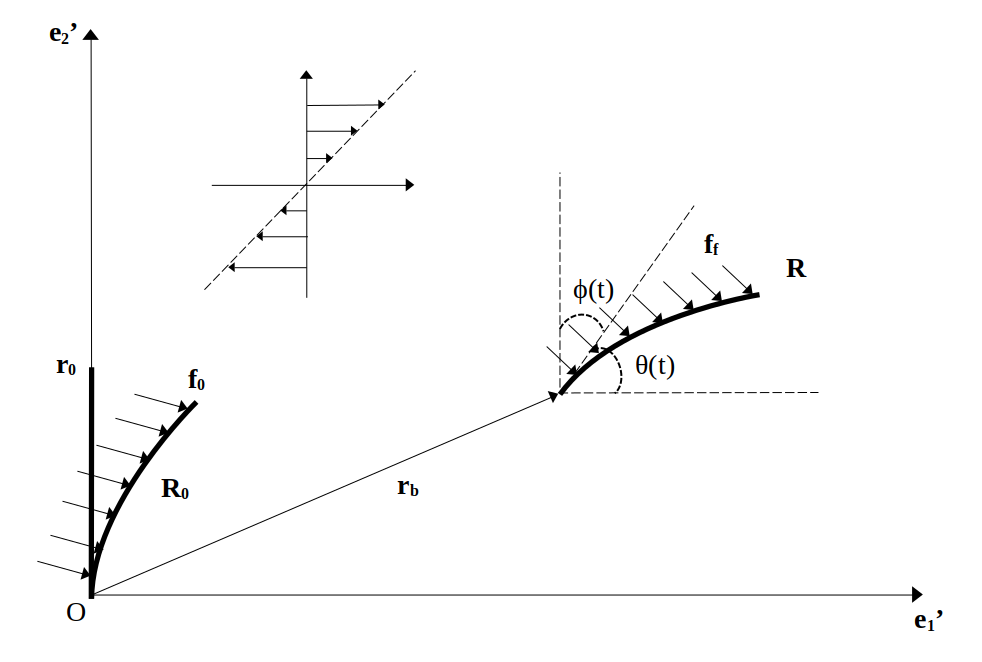
\includegraphics[width=1\textwidth]{plots/r0.png}
		\end{center}
		%	\setlength{\abovecaptionskip}{-0.5 cm}
	\end{figure}
\footnotesize Recall that 
\begin{equation*}
	\textbf{R}(t,\xi)=\mathbf{\mathcal{R}}\,\textbf{R}_0(\xi)+\textbf{r}_b(t),
\end{equation*}
\begin{equation*}
	\textbf{f}_{f}=\left(\mathbf{I}-\frac{1}{2}\textbf{e}_t\textbf{e}_t\right)\cdot(\textbf{U}^{\infty}-\textbf{U}).
\end{equation*}
	\column{.55\textwidth}
	\footnotesize
	Net drag and net torque: 
	\begin{equation*}
		\label{eqn:52}
		\textbf{F}=\int^1_0 \textbf{f}\, \left|\frac{\partial\textbf{R}}{\partial\xi}\right|\,d\xi, 
	\end{equation*}
	\begin{equation*}
		\label{eqn:53}
		\mathbf{T}\cdot\textbf{e}_z=\left\{\int^1_0 \left[(\textbf{R}-\textbf{R}_{centre})\times \textbf{f}\,\right]\,\left|\frac{\partial\textbf{R}}{\partial\xi}\right|\,d\xi\right\}\cdot\textbf{e}_z,
	\end{equation*}
	where 
	\begin{equation*}
		\label{eqn:54}
		\textbf{R}_{centre}=\int^1_0 \textbf{R}\,\Big|\frac{\partial\textbf{R}}{\partial\xi}\Big|\,d\xi.
	\end{equation*}
\vspace{0.1cm}

Drag-free and torque-free:
\begin{equation*}
	\textbf{F}\,(\textbf{R}_0(\xi), V, U_0, \phi_{eq})=\textbf{0},
\end{equation*}
\begin{equation*}
	\{\mathbf{T}\cdot\textbf{e}_z\}\,(\textbf{R}_0(\xi), V, U_0, \phi_{eq})=0.
\end{equation*} 
\end{columns}
	\end{overlayarea}
\end{frame}

%%%%%%%%%%%%%%%%%%%%%%%%%%%%%%%%%%%%%%%%%%%%%%%%%%%%%%%%%%%%%%%%%%%%%%


\begin{frame}
	\frametitle{Equilibrium equations}
	\begin{overlayarea}{\textwidth}{\textheight}
		\vspace{-0.8cm}
		\begin{columns}
			\column{.65\textwidth}
			\begin{figure}[htb]
				\begin{center}
					% specify width as 80% of the width of the text on the page
					% we can also specify a width in centimetres, e.g. [width=8cm]
					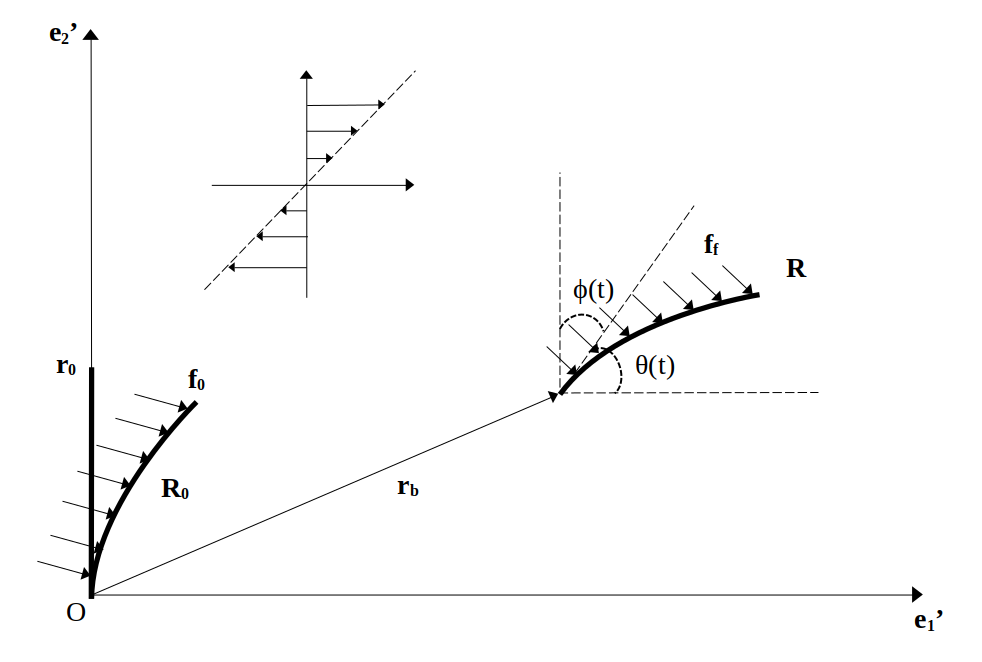
\includegraphics[width=1\textwidth]{plots/r0.png}
				\end{center}
				%	\setlength{\abovecaptionskip}{-0.5 cm}
			\end{figure}
			\footnotesize
			\begin{equation*}
				\left\{\begin{aligned}
					&\bm{\mathcal{S}}\left(\textbf{R}_0(\xi), V, U_0,\phi_{eq};\textbf{r}_0(\xi)\right)=0\\
					&\textbf{F}\,(\textbf{R}_0(\xi), V, U_0, \phi_{eq})=\textbf{0}\\
					&\{\mathbf{T}\cdot\textbf{e}_z\}\,(\textbf{R}_0(\xi), V, U_0, \phi_{eq})=0
				\end{aligned}\right.\Longrightarrow \left(\textbf{R}_0(\xi), V, U_0, \phi_{eq}\right).
			\end{equation*}
		\vspace{0.1cm}
		
		\tiny
		Recall that
		\begin{equation*}
			\int_0^1 \Bigg[ (\sigma_0 + \gamma) \delta \gamma 
			+ \frac{1}{12} h^2 \kappa \delta \kappa \Bigg. 
			\Bigg. - \Bigg( \frac{1}{h} \sqrt{\frac{A}{a}}\, \textbf{f}_s - \Lambda^2 \frac{\partial^2 \textbf{R}_0}{\partial t^2} \Bigg) 
			\cdot \delta \textbf{R}_0 \Bigg] \sqrt{a}\, d\xi = 0,
		\end{equation*}
			\column{.4\textwidth}
			\vspace{-2cm}
			\footnotesize
\begin{equation*}
	\textbf{f}_0=\mathcal{R}^{-1}\,\textbf{f}_f,
\end{equation*}
\begin{equation*}
	\textbf{f}_s=\mathcal{I}\,\textbf{f}_0=\mathcal{I}\,\left(\mathcal{R}^{-1}\,\textbf{f}_f\right),
\end{equation*}
where
 $$\mathbf{\mathcal{R}}=\left(\begin{aligned}
	&\cos(\phi_{eq})\quad -\sin((\phi_{eq}) \\
	&\sin((\phi_{eq})\quad \cos((\phi_{eq})
\end{aligned}\right). $$
		\end{columns}
	\end{overlayarea}
\end{frame}

%%%%%%%%%%%%%%%%%%%%%%%%%%%%%%%%%%%%%%%%%%%%%%%%%%%%%%%%%%%%%%%%%%%%%%



\begin{frame}
	\frametitle{Brief introduction of finite element method}
	\begin{overlayarea}{\textwidth}{\textheight}
		%\vspace{-0.8cm}
	%	\begin{columns}
		%	\column{.5\textwidth}
Let us consider a 1D problem: $\mathcal{R}(x;u(x))=0$, for $ x\in [0,1]$ subject to $u(x=0)=g_0, u(x=1)=g_1$.
\small\bi
\item Split the solution into two parts (Galerkin method): \vspace{-0.2cm}$$u(x)=u_p(x)+u_h(x)=u_p(x)+\sum^{N-1}_{j=2}U_j\psi_j(x).$$
($u_p(x=0)=g_0,u_p(x=1)=g_1$; $u_h(x=0)=u_h(x=1)=0$.)
\item Weak formulation (weak solution satisfies equation almost everywhere of domain): $$r_k(U_2,U_3,...,U_{N-1})=\int^1_0\mathcal{R}\Bigg(u_p(x)+\sum^{N-1}_{j=2}U_j\psi_j(x)\Bigg)\,\psi_k(x)\,dx.$$
\item Note that $\{U_2,U_3,...U_{N-1}\}$ are the unknowns. 
\ei
	
	
			%\column{.5\textwidth}

		%\end{columns}
	\end{overlayarea}
\end{frame}

%%%%%%%%%%%%%%%%%%%%%%%%%%%%%%%%%%%%%%%%%%%%%%%%%%%%%%%%%%%%%%%%%%%%%%



\begin{frame}
	\frametitle{Brief introduction of finite element method}
	\begin{overlayarea}{\textwidth}{\textheight}
\vspace{-0.2cm}\small	Shape functions: "hat functions".
$$\psi_j(x)=
\begin{cases}
	0 & \text{for}\quad x<X_{j-1} \\
	\frac{x-X_{j-1}}{X_{j}-X_{j-1}} & \text{for}\quad X_{j-1}<x<X_{j}\\
	\frac{X_{j+1}-x}{X_{j+1}-X_{j}} & \text{for}\quad X_{j}<x<X_{j+1} \\
	0 & \text{for}\quad x>X_{j+1}
\end{cases}$$\vspace{-0.6cm}
\begin{figure}[htb]
	\begin{minipage}[t]{0.49\linewidth}
		\centering
		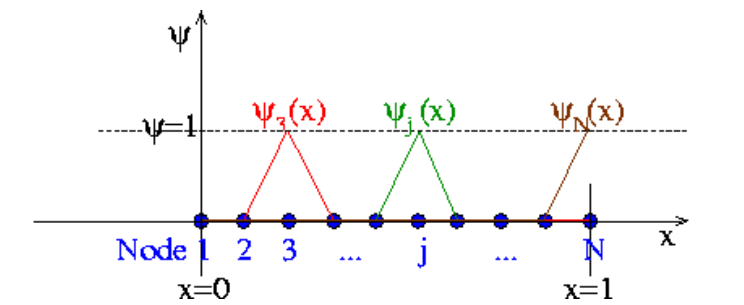
\includegraphics[scale=0.22]{plots/finite1.png}
	\end{minipage}
	\begin{minipage}[t]{0.49\linewidth}
		\centering
		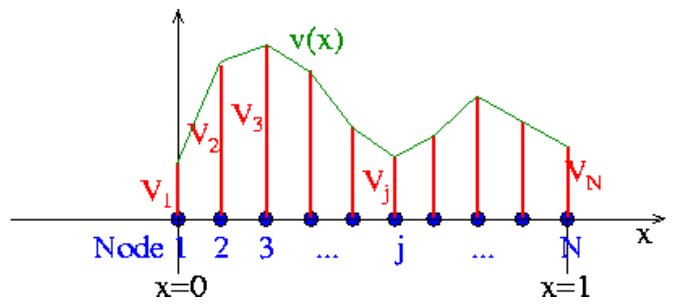
\includegraphics[scale=0.22]{plots/finite2.png}
	\end{minipage}
\end{figure}\vspace{-0.2cm}
\bi
\item Shape functions satisfy $\psi_j(X_i)=
\begin{cases}
	1 & \text{if}\quad i=j \\
	0 & \text{for}\quad i\neq j
\end{cases}.$
\item Piecewise linear interpolation $v(x)=\sum^N_{j=1} V_j \psi_j(x)$.
\ei
		\end{overlayarea}
	\end{frame}
	
	%%%%%%%%%%%%%%%%%%%%%%%%%%%%%%%%%%%%%%%%%%%%%%%%%%%%%%%%%%%%%%%%%%%%%%



\begin{frame}
	\frametitle{Newton method}
	\begin{overlayarea}{\textwidth}{\textheight}
		\vspace{-0.5cm}\small	
		\bi
		\item Set $u_p=g_0\psi_1(x)+g_1\psi_N(x)$ and $\sum^{N-1}_{j=2}U_j\psi_j(x)$.
		\item Provide an initial guess for the unknowns $\{U_2,U_3,...U_{N-1}\}$, denoted as $U_i^{(0)}, i=2,...,N-1.$
		\item Determine the residuals $$r_k^{(0)}=\int^1_0\mathcal{R}\Bigg(u_p(x)+\sum^{N-1}_{j=2}U_j\psi_j(x)\Bigg)\,\psi_k(x)\,dx,\, k=2,...,N-1.$$
	 and the entries in the Jacobian matrix $J_{kj}=\frac{\partial r_k}{\partial U_j},\, k,j=2,...,N-1.$
	 \item Solve the linear system $\sum^{N-1}_{j=2}J_{kj}\,\delta U_j=-r_k^{(0)},\,k=2,...,N-1.$
	 \item Correct the initial guess via $U_j=U_j^{(0)}+\delta U_j,\, j=2,...,N-1.$ 
	 \item The finite-element solution is\vspace{-0.2cm} $$u^{(FE)}(x)=g_0\psi_1(x)+g_1\psi_N(x)+\sum^{N-1}_{j=2}U_j\psi_j(x).$$
		\ei
	\end{overlayarea}
\end{frame}

%%%%%%%%%%%%%%%%%%%%%%%%%%%%%%%%%%%%%%%%%%%%%%%%%%%%%%%%%%%%%%%%%%%%%%

\begin{frame}
	\frametitle{Geometry}
	\begin{overlayarea}{\textwidth}{\textheight}
		\vspace{-0.3cm}	
	\begin{itemize}
		\item  Based on the rigid case results from Roggeveen and Stone’s paper (2D).
		\item Rigid:\vspace{-0.3cm}
		\begin{figure}[htb]
			\begin{center}
				% specify width as 80% of the width of the text on the page
				% we can also specify a width in centimetres, e.g. [width=8cm]
				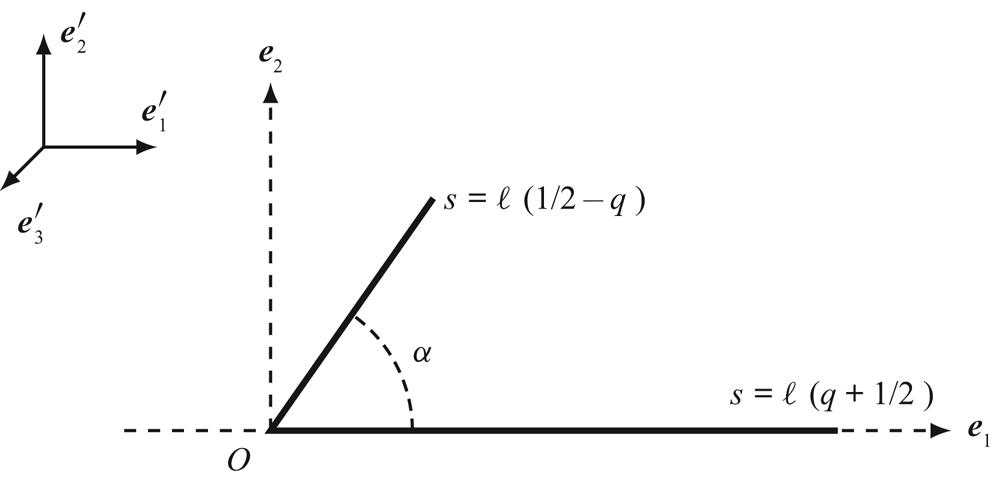
\includegraphics[width=0.5\textwidth]{plots/stone2.png}
			\end{center}
			%	\setlength{\abovecaptionskip}{-0.5 cm}
		\end{figure}
		\item Elastic (initial configuration):
		\begin{figure}[htb]
			\begin{center}
				% specify width as 80% of the width of the text on the page
				% we can also specify a width in centimetres, e.g. [width=8cm]
				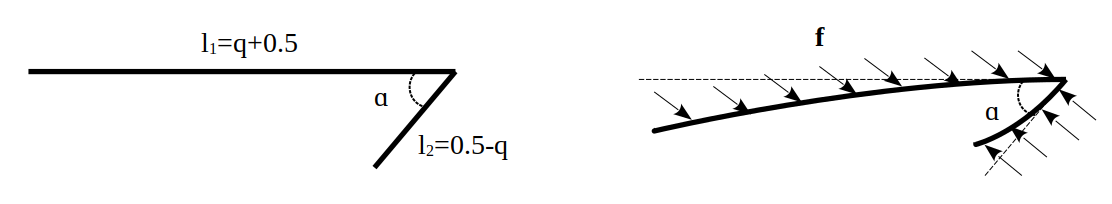
\includegraphics[width=0.8\textwidth]{plots/geometry.png}
			\end{center}
			%	\setlength{\abovecaptionskip}{-0.5 cm}
		\end{figure}\vspace{-0.2cm}
	\item Base and develop the code in \texttt{oomph-lib}\footnote{\texttt{oomph-lib} is an object-oriented, open-source finite-element library for the simulation of multi-physics problems.}.
		%\selectfont \fontsize{10}{15}\selectfont
	\end{itemize}
	\end{overlayarea}
\end{frame}

%%%%%%%%%%%%%%%%%%%%%%%%%%%%%%%%%%%%%%%%%%%%%%%%%%%%%%%%%%%%%%%%%%%%%%

\begin{frame}
	\frametitle{Results}
	\begin{overlayarea}{\textwidth}{\textheight}
		\vspace{-0.3cm}
	Fixed points: \small Of these four fixed orientations, two differ from the other two by an angle of $\pi$ but possess the same shapes.
	\begin{itemize} 
		\item rigid:
		\vspace{-0.3cm}
		\begin{figure}[htb]
			\begin{center}
				% specify width as 80% of the width of the text on the page
				% we can also specify a width in centimetres, e.g. [width=8cm]
				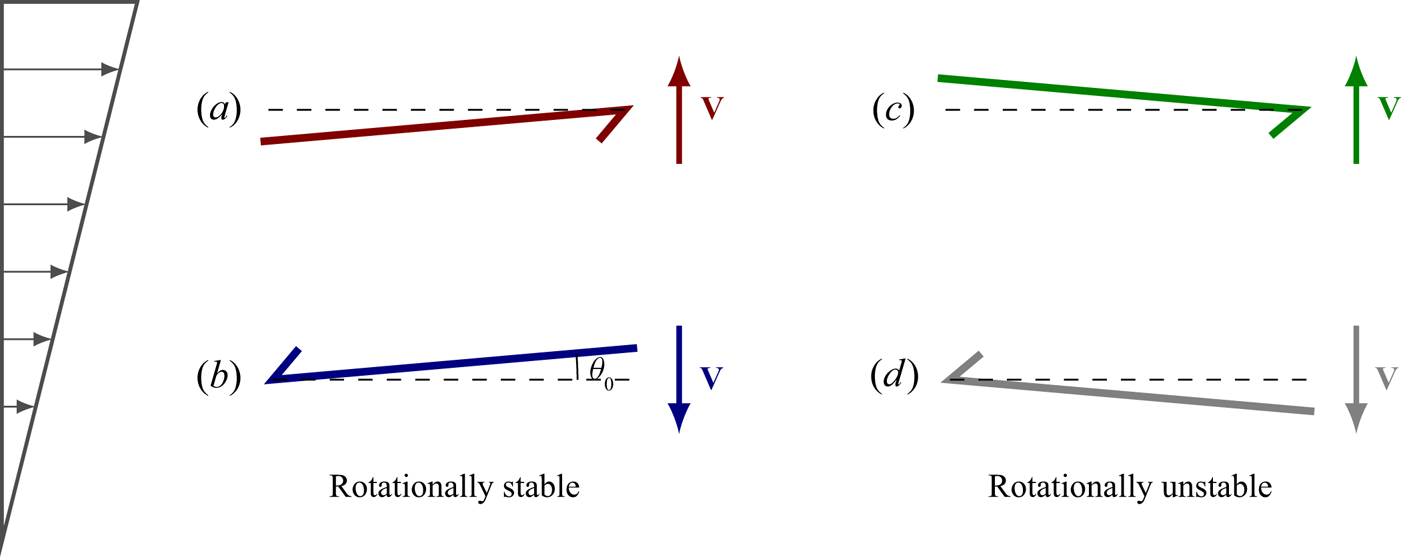
\includegraphics[width=0.6\textwidth]{plots/stone3.png}
			\end{center}
			%	\setlength{\abovecaptionskip}{-0.5 cm}
		\end{figure}\vspace{-0.3cm}
		\item elastic:\vspace{-0.3cm}
		\begin{figure}[htb]
			\begin{center}
				% specify width as 80% of the width of the text on the page
				% we can also specify a width in centimetres, e.g. [width=8cm]
				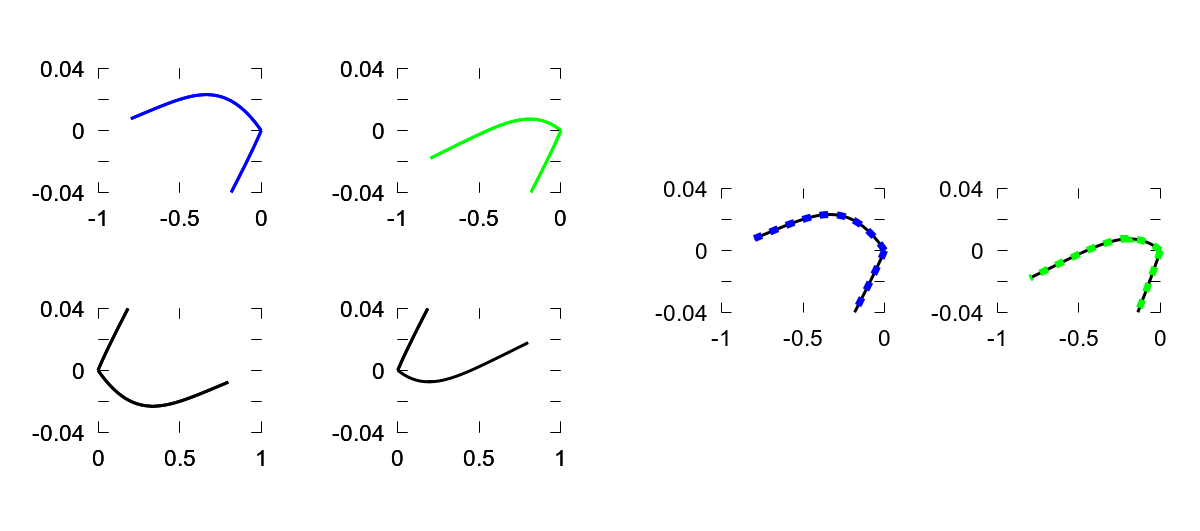
\includegraphics[width=0.7\textwidth]{plots/four_solutions2.png}
			\end{center}
			%	\setlength{\abovecaptionskip}{-0.5 cm}
		\end{figure}   
		%\selectfont \fontsize{10}{15}\selectfont
	\end{itemize}
	\end{overlayarea}
\end{frame}

%%%%%%%%%%%%%%%%%%%%%%%%%%%%%%%%%%%%%%%%%%%%%%%%%%%%%%%%%%%%%%%%%%%%%%


\begin{frame}
	\frametitle{Results}
	\begin{overlayarea}{\textwidth}{\textheight}
	\begin{itemize}
		\item $q=0.3, \alpha=0.125\pi$.
		\begin{figure}[htb]
			\begin{center}
				% specify width as 80% of the width of the text on the page
				% we can also specify a width in centimetres, e.g. [width=8cm]
				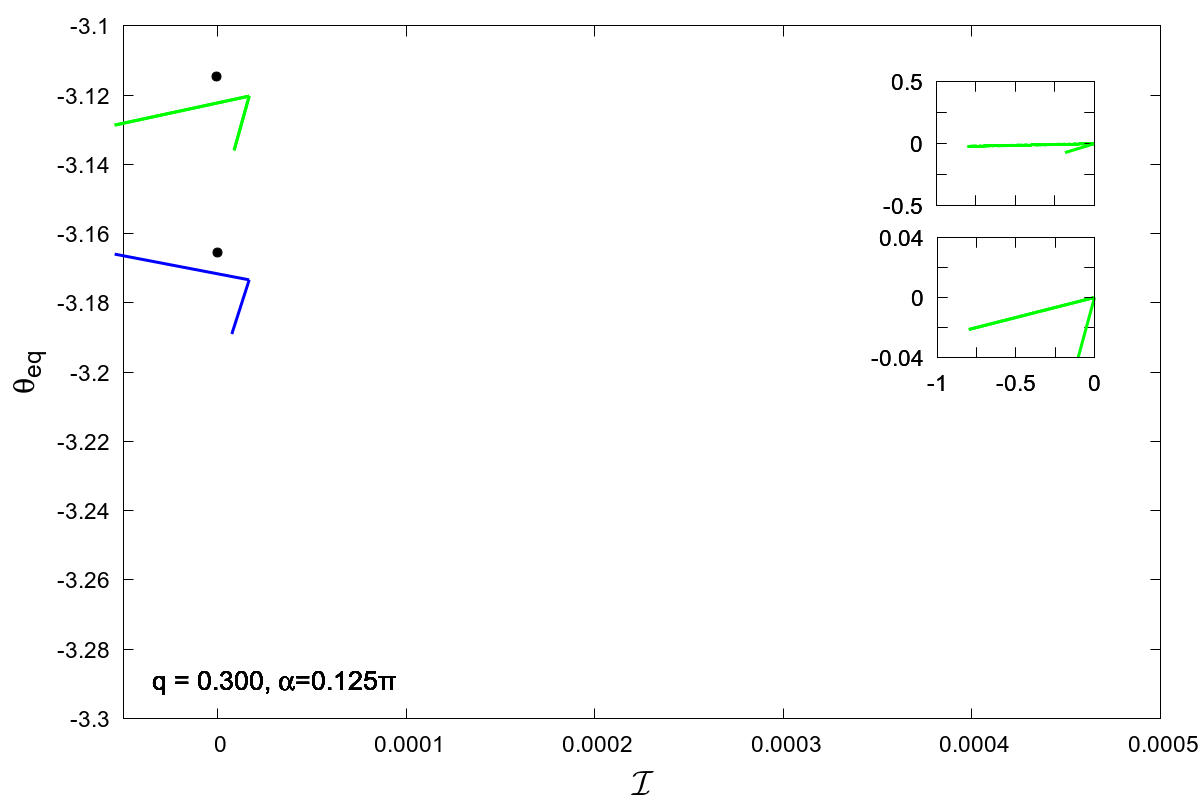
\includegraphics[width=0.9\textwidth]{plots/combine_elastic_beam_I_theta_q_0.30_alpha_0.125pi_initial_-4.80_0.png}
			\end{center}
			%	\setlength{\abovecaptionskip}{-0.5 cm}
		\end{figure}
		%\selectfont \fontsize{10}{15}\selectfont
	\end{itemize}
	\end{overlayarea}
\end{frame}

%%%%%%%%%%%%%%%%%%%%%%%%%%%%%%%%%%%%%%%%%%%%%%%%%%%%%%%%%%%%%%%%%%%%%%

\begin{frame}
	\frametitle{Results}
	\begin{overlayarea}{\textwidth}{\textheight}
	\begin{itemize}
		\item $q=0.44, \alpha=0.125\pi$.
		\begin{figure}[htb]
			\begin{center}
				% specify width as 80% of the width of the text on the page
				% we can also specify a width in centimetres, e.g. [width=8cm]
				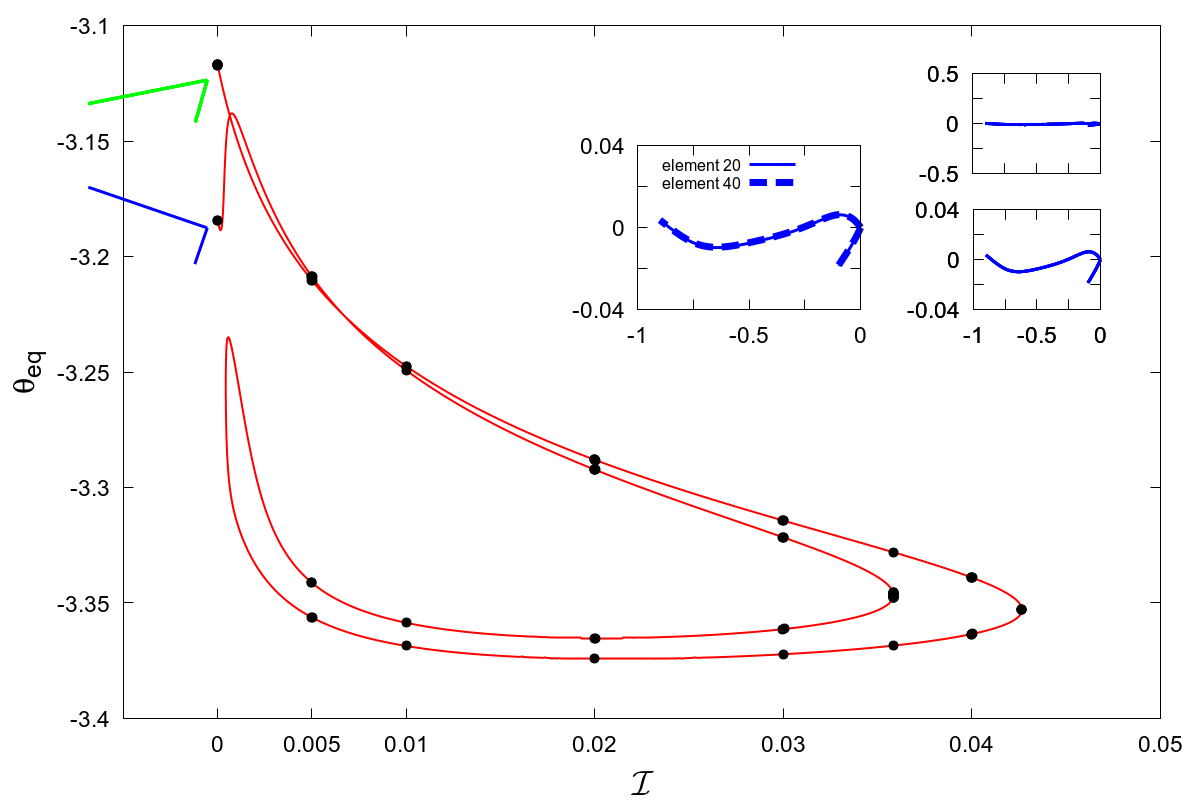
\includegraphics[width=0.9\textwidth]{plots/combine_elastic_beam_I_theta_q_0.400_alpha_0.125pi_initial_-4.80_0.png}
			\end{center}
			%	\setlength{\abovecaptionskip}{-0.5 cm}
		\end{figure}
		%\selectfont \fontsize{10}{15}\selectfont
	\end{itemize}
	\end{overlayarea}
\end{frame}

%%%%%%%%%%%%%%%%%%%%%%%%%%%%%%%%%%%%%%%%%%%%%%%%%%%%%%%%%%%%%%%%%%%%%%

\begin{frame}
	\frametitle{Results}
	\begin{overlayarea}{\textwidth}{\textheight}
\begin{itemize}
	\item $q=0.44, \alpha=0.125\pi$ (logarithmic plot).
	\begin{figure}[htb]
		\begin{center}
			% specify width as 80% of the width of the text on the page
			% we can also specify a width in centimetres, e.g. [width=8cm]
			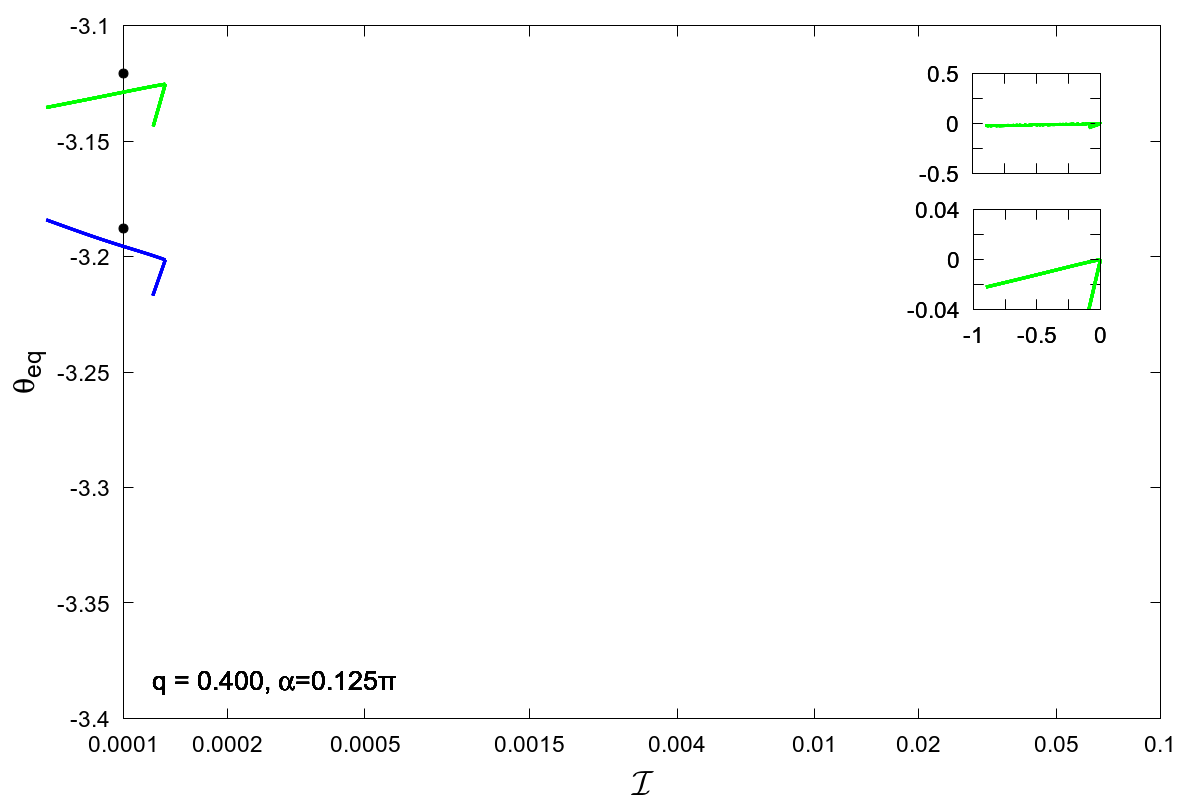
\includegraphics[width=0.9\textwidth]{plots/initial_combine_elastic_beam_I_theta_q_0.400_alpha_0.125pi_initial_-4.80_0.png}
		\end{center}
		%	\setlength{\abovecaptionskip}{-0.5 cm}
	\end{figure}
	%\selectfont \fontsize{10}{15}\selectfont
\end{itemize}
	\end{overlayarea}
\end{frame}

%%%%%%%%%%%%%%%%%%%%%%%%%%%%%%%%%%%%%%%%%%%%%%%%%%%%%%%%%%%%%%%%%%%%%%


\begin{frame}
	\frametitle{Results}
	\begin{overlayarea}{\textwidth}{\textheight}
\begin{itemize}
	\item $q=0.44, \alpha=0.125\pi$.
	\begin{figure}[htb]
		\begin{center}
			% specify width as 80% of the width of the text on the page
			% we can also specify a width in centimetres, e.g. [width=8cm]
			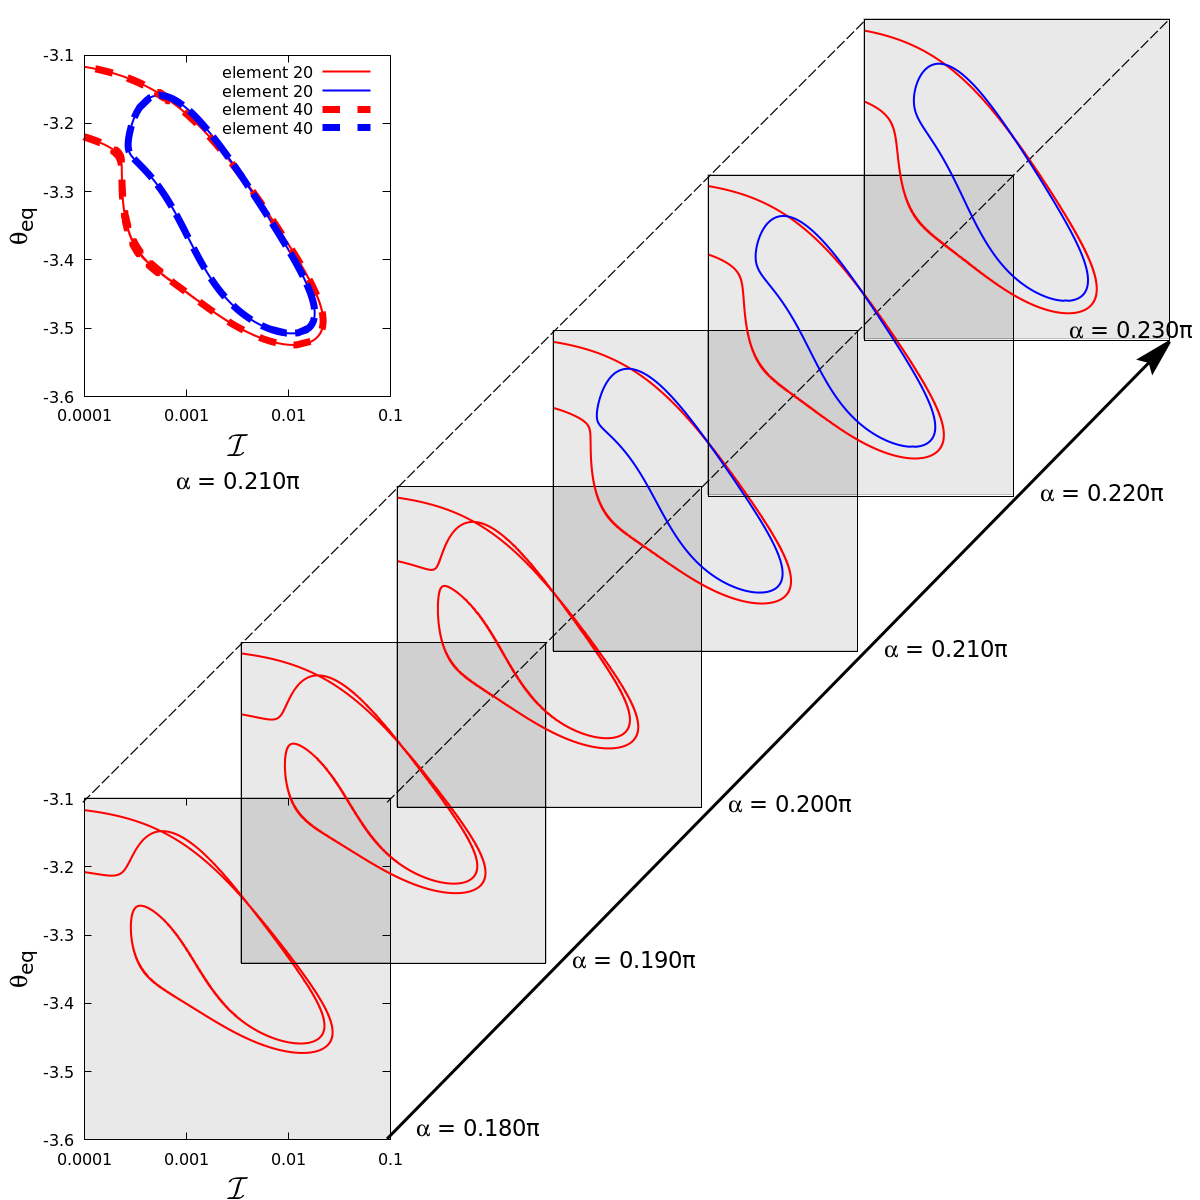
\includegraphics[width=0.65\textwidth]{plots/elastic_beam_I_theta_q_0.400_alpha.png}
		\end{center}
		%	\setlength{\abovecaptionskip}{-0.5 cm}
	\end{figure}
	%\selectfont \fontsize{10}{15}\selectfont
\end{itemize}
	\end{overlayarea}
\end{frame}

%%%%%%%%%%%%%%%%%%%%%%%%%%%%%%%%%%%%%%%%%%%%%%%%%%%%%%%%%%%%%%%%%%%%%%



\begin{frame}
	\frametitle{Results}
	\begin{overlayarea}{\textwidth}{\textheight}
\begin{itemize}
	\item $q=0.452, \alpha=0.125\pi$.
	\begin{figure}[htb]
		\begin{center}
			% specify width as 80% of the width of the text on the page
			% we can also specify a width in centimetres, e.g. [width=8cm]
			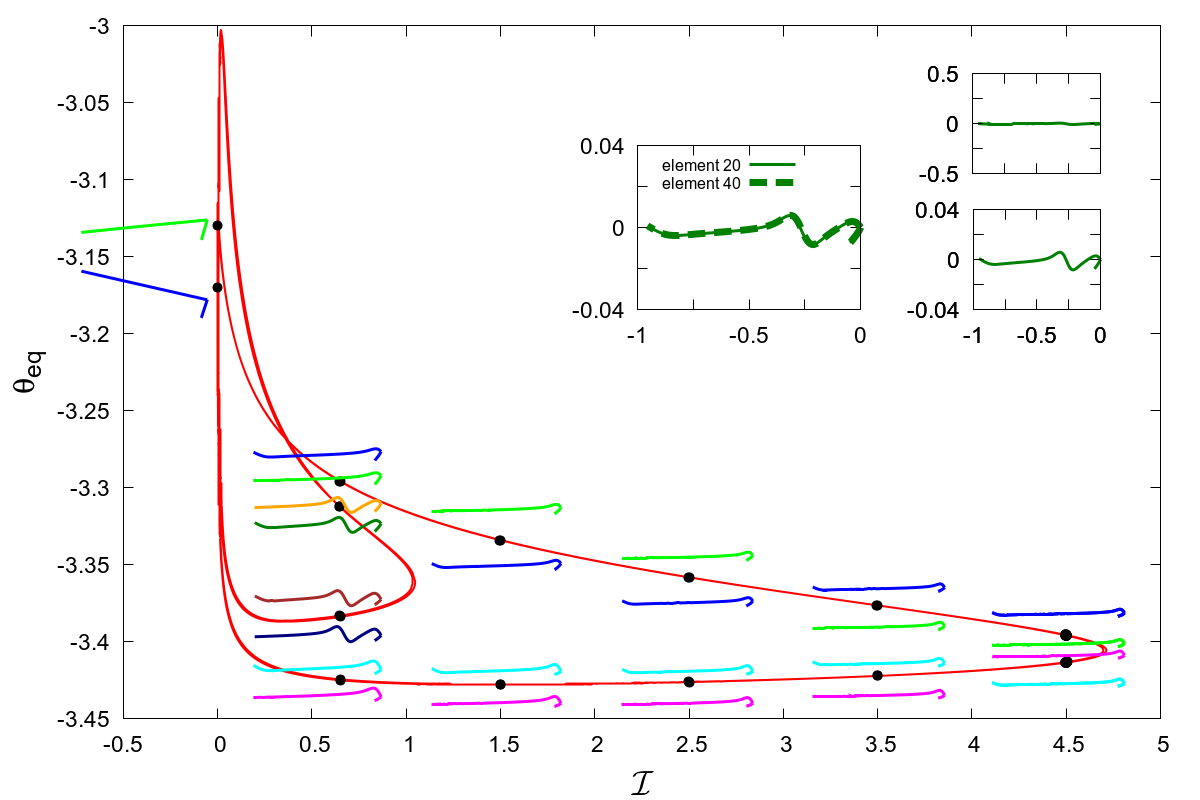
\includegraphics[width=0.9\textwidth]{plots/combine_elastic_beam_I_theta_q_0.452_alpha_0.125pi_initial_-4.80_0.png}
		\end{center}
		%	\setlength{\abovecaptionskip}{-0.5 cm}
	\end{figure}
	%\selectfont \fontsize{10}{15}\selectfont
\end{itemize}
	\end{overlayarea}
\end{frame}

%%%%%%%%%%%%%%%%%%%%%%%%%%%%%%%%%%%%%%%%%%%%%%%%%%%%%%%%%%%%%%%%%%%%%%




\begin{frame}
	\frametitle{Results}
	\begin{overlayarea}{\textwidth}{\textheight}
	\begin{itemize}
		\item $q=0.452, \alpha\in [0.120\pi, 0.
		170\pi]$.
		\begin{figure}[htb]
			\begin{center}
				% specify width as 80% of the width of the text on the page
				% we can also specify a width in centimetres, e.g. [width=8cm]
				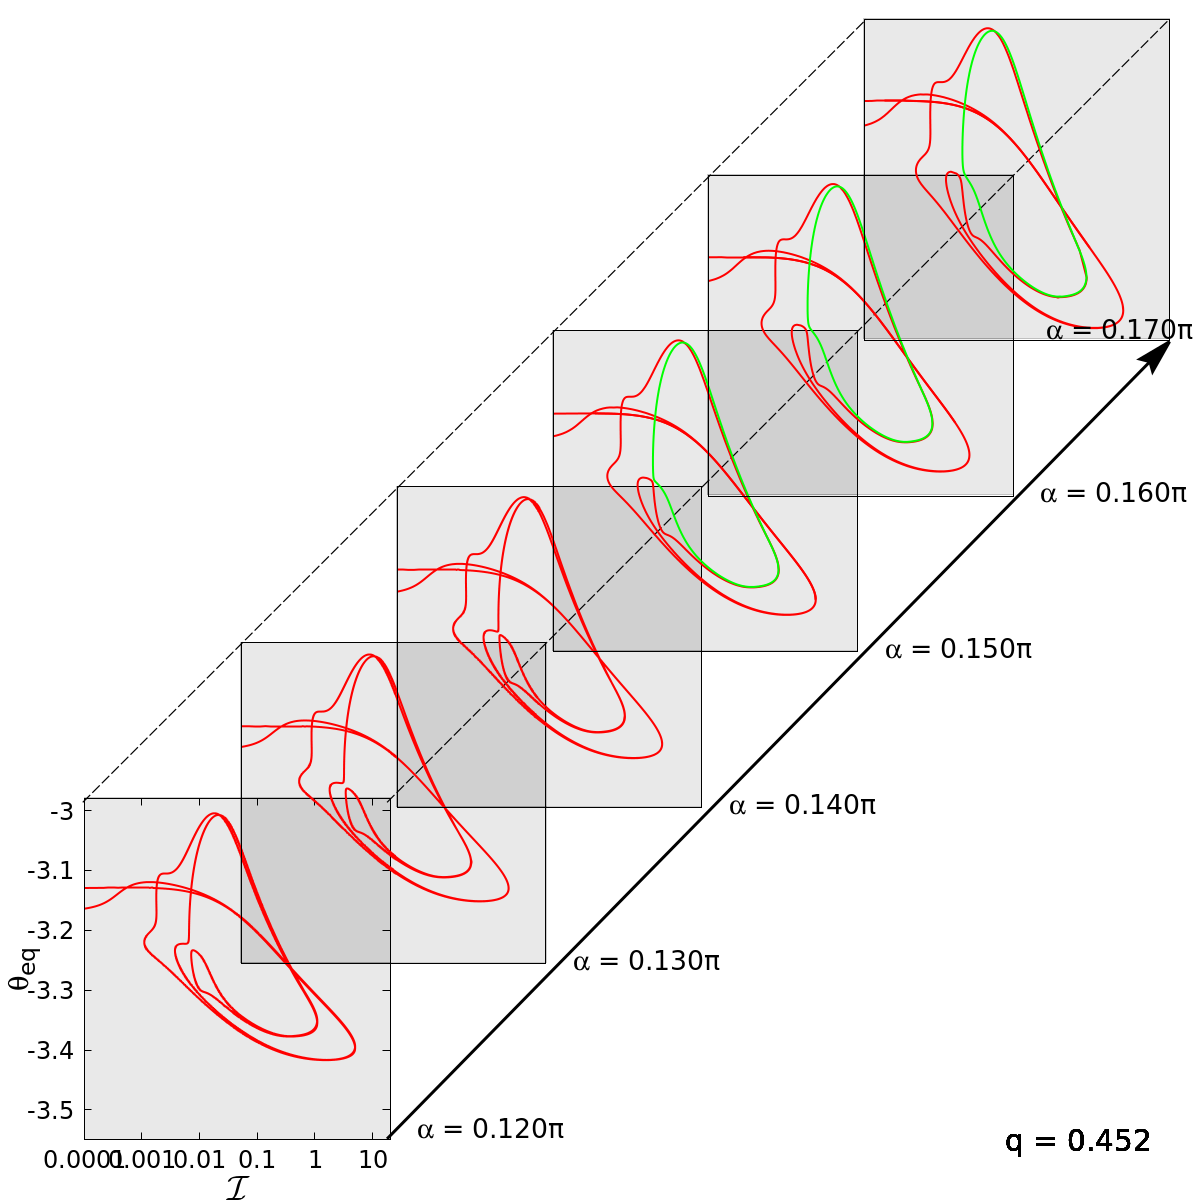
\includegraphics[width=0.65\textwidth]{plots/elastic_beam_I_theta_q_0.452_alpha_restart1.png}
			\end{center}
			%	\setlength{\abovecaptionskip}{-0.5 cm}
		\end{figure}
		%\selectfont \fontsize{10}{15}\selectfont
	\end{itemize}
	\end{overlayarea}
\end{frame}

%%%%%%%%%%%%%%%%%%%%%%%%%%%%%%%%%%%%%%%%%%%%%%%%%%%%%%%%%%%%%%%%%%%%%%


\begin{frame}
	\frametitle{Results}
	\begin{overlayarea}{\textwidth}{\textheight}
		\begin{itemize}
			\item $q=0.452, \alpha\in [0.250\pi, 0.
			300\pi]$.
			\begin{figure}[htb]
				\begin{center}
					% specify width as 80% of the width of the text on the page
					% we can also specify a width in centimetres, e.g. [width=8cm]
					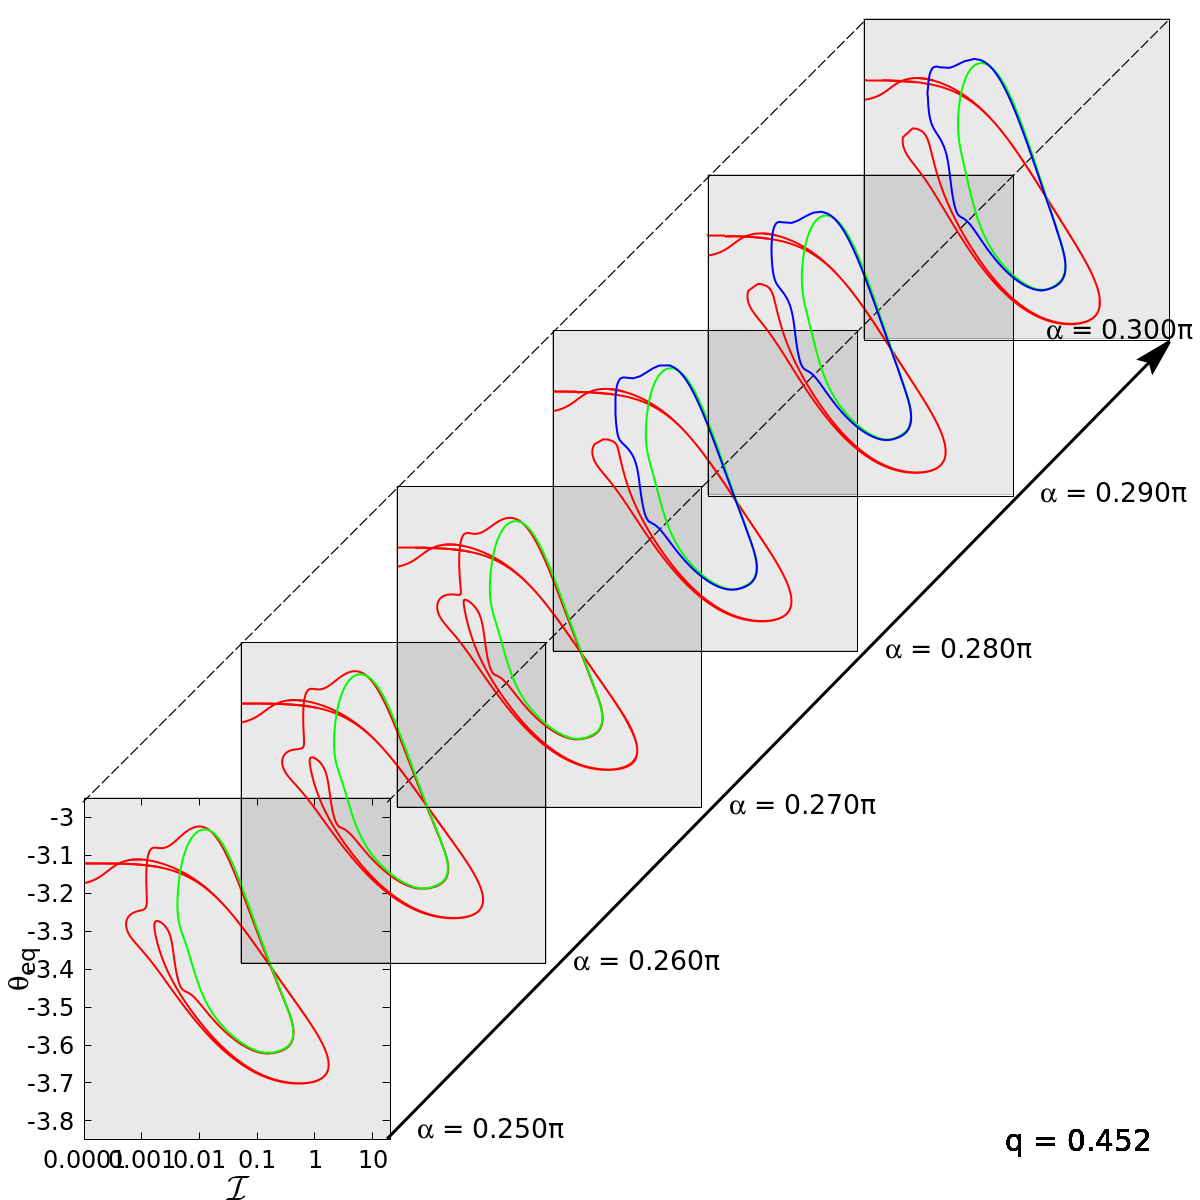
\includegraphics[width=0.65\textwidth]{plots/elastic_beam_I_theta_q_0.452_alpha_restart2.png}
				\end{center}
				%	\setlength{\abovecaptionskip}{-0.5 cm}
			\end{figure}
			%\selectfont \fontsize{10}{15}\selectfont
		\end{itemize}
	\end{overlayarea}
\end{frame}

%%%%%%%%%%%%%%%%%%%%%%%%%%%%%%%%%%%%%%%%%%%%%%%%%%%%%%%%%%%%%%%%%%%%%%


\begin{frame}
	\frametitle{Results}
	\begin{overlayarea}{\textwidth}{\textheight}
\begin{itemize}
	\item $q=0.452, \alpha\in [0.370\pi, 0.
420\pi]$.
	\begin{figure}[htb]
		\begin{center}
			% specify width as 80% of the width of the text on the page
			% we can also specify a width in centimetres, e.g. [width=8cm]
			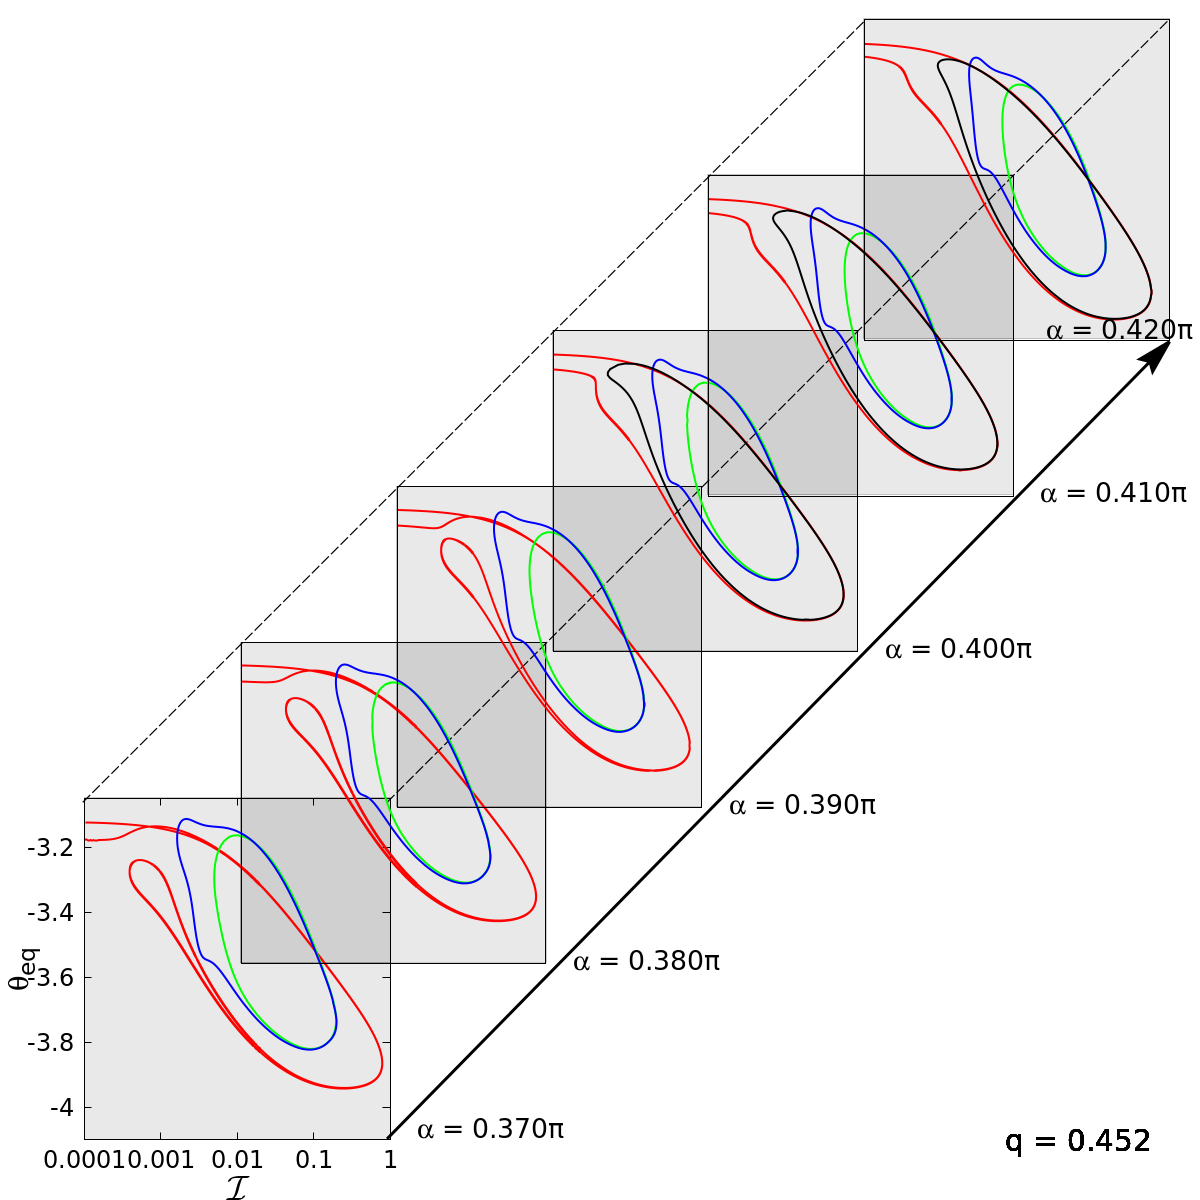
\includegraphics[width=0.65\textwidth]{plots/elastic_beam_I_theta_q_0.452_alpha_restart3.png}
		\end{center}
		%	\setlength{\abovecaptionskip}{-0.5 cm}
	\end{figure}
	%\selectfont \fontsize{10}{15}\selectfont
\end{itemize}
	\end{overlayarea}
\end{frame}

%%%%%%%%%%%%%%%%%%%%%%%%%%%%%%%%%%%%%%%%%%%%%%%%%%%%%%%%%%%%%%%%%%%%%%


\begin{frame}
	\frametitle{Results}
	\begin{overlayarea}{\textwidth}{\textheight}
\begin{itemize}
	\item Four types of deformations: \vspace{-0.3cm}
	\begin{figure}[htb]
		\begin{center}
			% specify width as 80% of the width of the text on the page
			% we can also specify a width in centimetres, e.g. [width=8cm]
			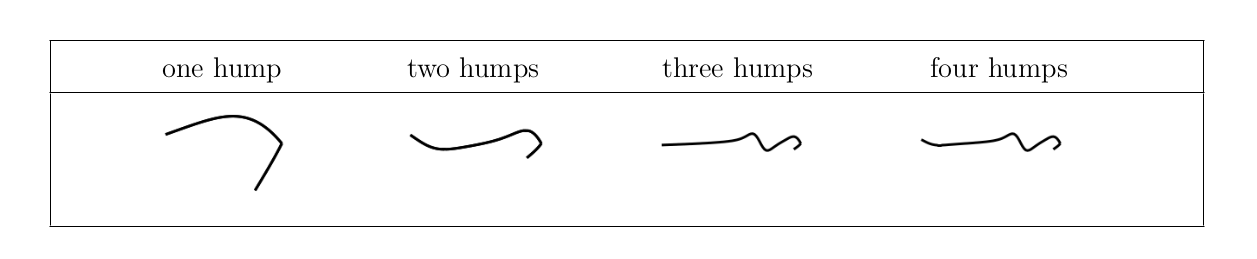
\includegraphics[width=1\textwidth]{plots/deformations.png}
		\end{center}
		%	\setlength{\abovecaptionskip}{-0.5 cm}
	\end{figure}
	\item Note that the initial configurations are the boomerang shapes.
		\begin{figure}[htb]
		\begin{center}
			% specify width as 80% of the width of the text on the page
			% we can also specify a width in centimetres, e.g. [width=8cm]
			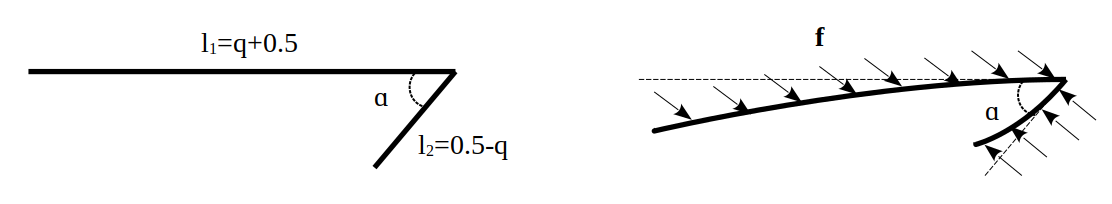
\includegraphics[width=0.8\textwidth]{plots/geometry.png}
		\end{center}
		%	\setlength{\abovecaptionskip}{-0.5 cm}
	\end{figure}
	\item The initial configuration ($q,\alpha$) plays a crucial role in the deformations.
	%\selectfont \fontsize{10}{15}\selectfont
\end{itemize}
	\end{overlayarea}
\end{frame}

%%%%%%%%%%%%%%%%%%%%%%%%%%%%%%%%%%%%%%%%%%%%%%%%%%%%%%%%%%%%%%%%%%%%%%



\begin{frame}
	\frametitle{Results}
	\begin{overlayarea}{\textwidth}{\textheight}
	\begin{itemize}
		\item Rigid case results from Roggeveen and Stone’s paper:
		\begin{columns}
			\begin{column}{0.5\textwidth}
			\begin{figure}[htb]
				\begin{center}
					% specify width as 80% of the width of the text on the page
					% we can also specify a width in centimetres, e.g. [width=8cm]
					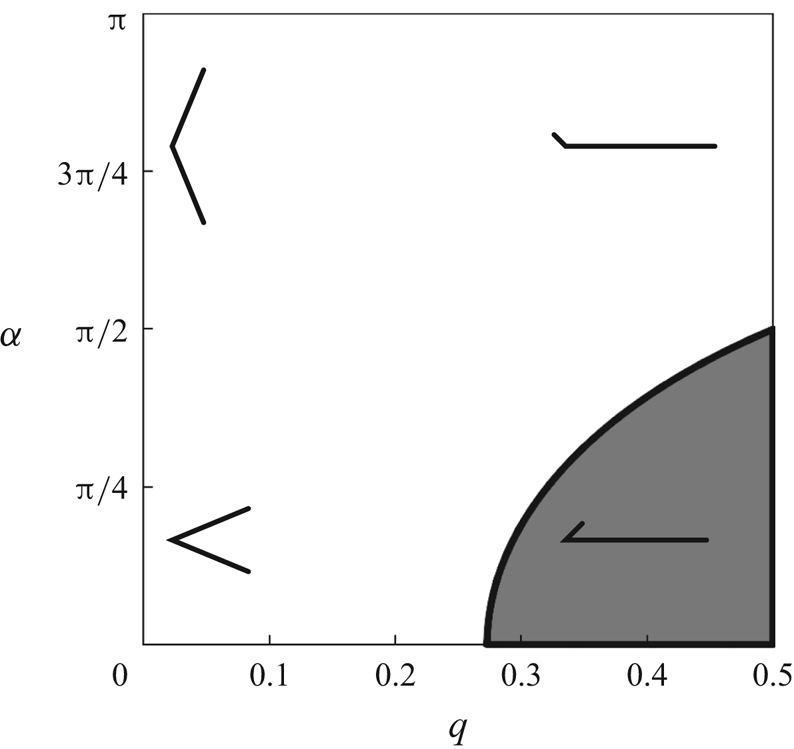
\includegraphics[width=1\textwidth]{plots/stone.png}
				\end{center}
				%	\setlength{\abovecaptionskip}{-0.5 cm}
			\end{figure}
			\end{column}
			\begin{column}{0.5\textwidth}
				Gray region represents the bodies for which fixed points exist.
			\end{column}
		\end{columns}
		\item Since the initial configurations significantly influence deformations, we aim to plot a similar figure to illustrate which types of initial configurations lead to fixed orientations.
	\end{itemize}
	\end{overlayarea}
\end{frame}

%%%%%%%%%%%%%%%%%%%%%%%%%%%%%%%%%%%%%%%%%%%%%%%%%%%%%%%%%%%%%%%%%%%%%%

\begin{frame}
	\frametitle{Results}
	\begin{overlayarea}{\textwidth}{\textheight}
\begin{itemize}
	\item $q=0.4$.
	\begin{figure}
		\begin{minipage}{0.49\linewidth}
			\centering
			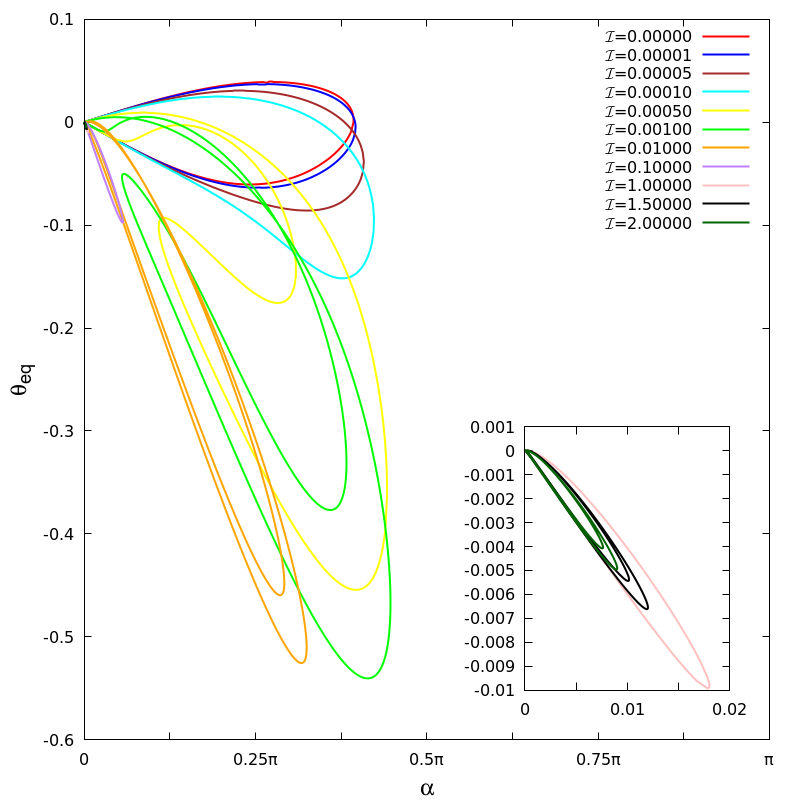
\includegraphics[width=\linewidth]{plots/elastic_beam_alpha_theta_eq_q_0.400.png} 
		\end{minipage}
		\hfill
		\begin{minipage}{0.49\linewidth}
			\centering
			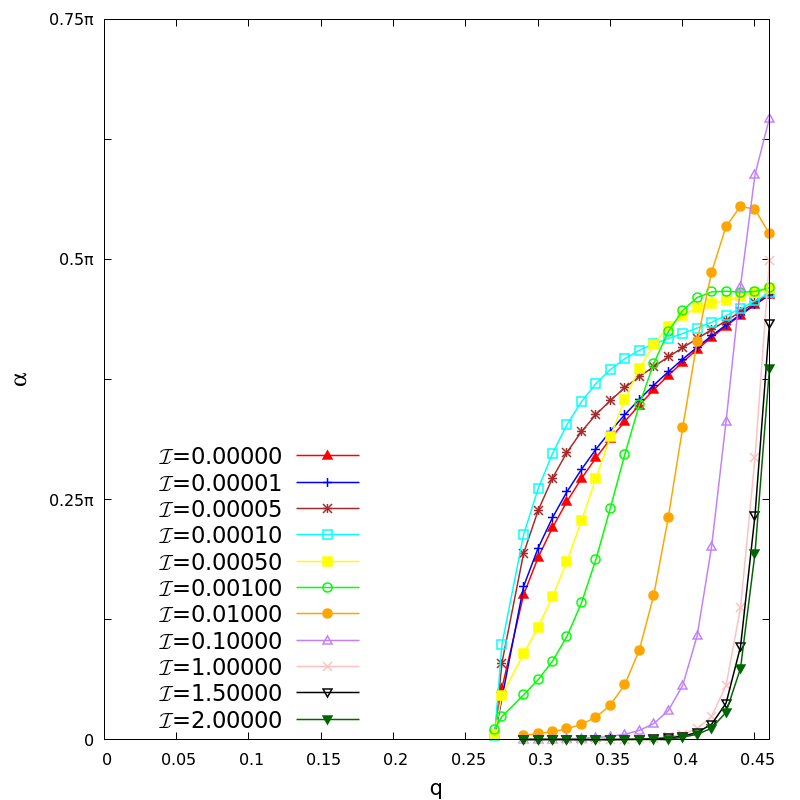
\includegraphics[width=\linewidth]{plots/elastic_beam_general.png} 
		\end{minipage}
	\end{figure}
	
	%\selectfont \fontsize{10}{15}\selectfont
\end{itemize}
	\end{overlayarea}
\end{frame}

%%%%%%%%%%%%%%%%%%%%%%%%%%%%%%%%%%%%%%%%%%%%%%%%%%%%%%%%%%%%%%%%%%%%%%


\begin{frame}
	\frametitle{Results}
	\begin{overlayarea}{\textwidth}{\textheight}
		\vspace{-0.3cm}
	\begin{itemize}
		\item \small Define the tensile stress for rigid particles as 
		\begin{equation*}
			\sigma(\xi)=\int_0^\xi (\mathbf{f}\cdot\mathbf{t}) \left |\frac{\partial \mathbf{R}}{\partial \xi}\right|\,d\xi,
		\end{equation*}
		where $\mathbf{t}$ is the unit tangent vector to the surface of the particle. 
	\item \small Therefore, we have 
	\begin{equation*}\small 
		\sigma(\xi)=\left\{
		\begin{aligned}
			\label{eq:4}
			&\int_0^\xi (\mathbf{f}\cdot\mathbf{t}_1) \left |\frac{\partial \mathbf{R}}{\partial \xi}\right|\,d\xi,\quad \xi\in[0,0.5-q];\\
			&-\mathbf{F}_2\cdot\mathbf{t}_2+\int_{0.5-q}^\xi (\mathbf{f}\cdot\mathbf{t}_2) \left |\frac{\partial \mathbf{R}}{\partial \xi}\right|\,d\xi, \quad \xi\in[0.5-q,1].
		\end{aligned}\right.
	\end{equation*}
	\end{itemize}\vspace{-0.4cm}
	\begin{figure}[htb]
	\begin{center}
		% specify width as 80% of the width of the text on the page
		% we can also specify a width in centimetres, e.g. [width=8cm]
		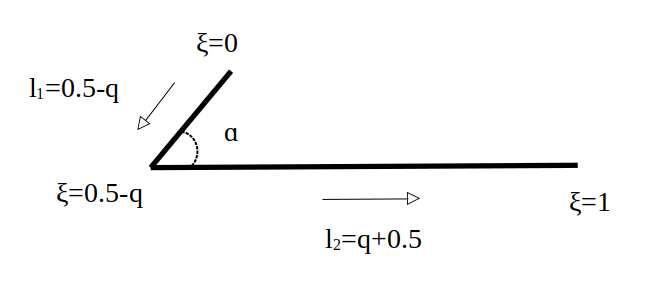
\includegraphics[width=0.55\textwidth]{plots/tensile_boomerang.png}
	\end{center}
	%	\setlength{\abovecaptionskip}{-0.5 cm}
\end{figure}
	\end{overlayarea}
\end{frame}

%%%%%%%%%%%%%%%%%%%%%%%%%%%%%%%%%%%%%%%%%%%%%%%%%%%%%%%%%%%%%%%%%%%%%%

\begin{frame}
	\frametitle{Results}
	\begin{overlayarea}{\textwidth}{\textheight}
Tensile stress for different shape parameters ($\mathcal{I}=0$).\vspace{-0.2cm}
\begin{figure}[!h]
	\centering
	\subfigure[\tiny $q=0.35,\alpha=0.125\pi$]{
		\begin{minipage}[b]{0.25\textwidth}
			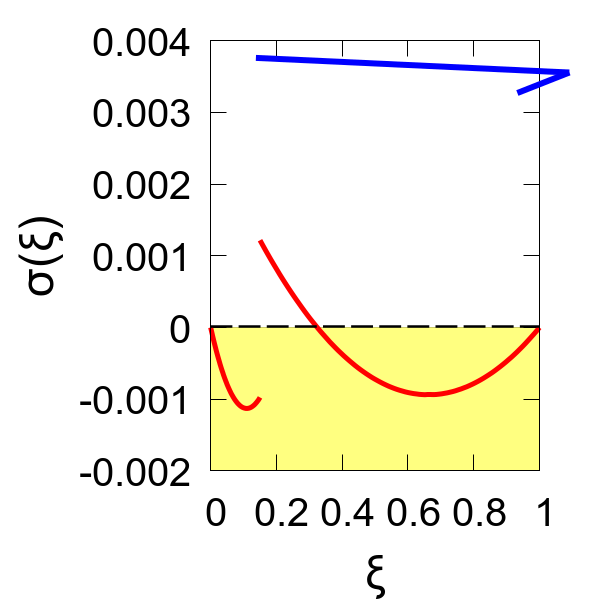
\includegraphics[width=1\textwidth]{plots/sigma_q_0.35_alpha_0.125pi.png} 
		\end{minipage}
		\label{fig:10.a}
	}
	\subfigure[\tiny $q=0.40,\alpha=0.125\pi$]{
		\begin{minipage}[b]{0.25\textwidth}
			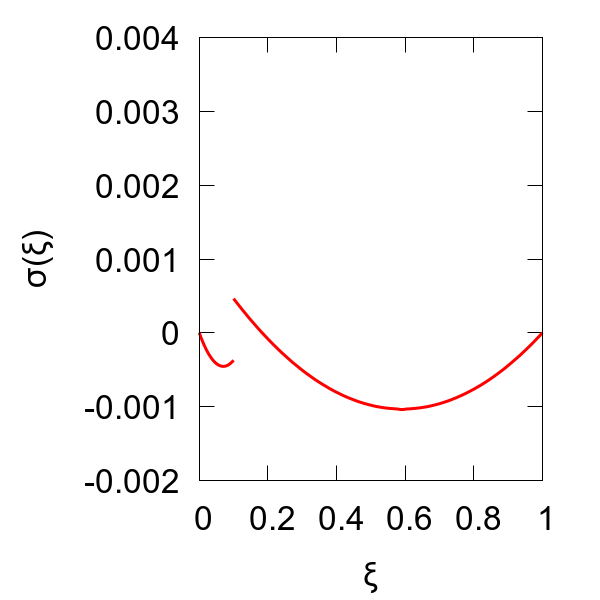
\includegraphics[width=1\textwidth]{plots/sigma_q_0.4_alpha_0.125pi.png}
		\end{minipage}
		\label{fig:10.b}
	}
	\subfigure[\tiny $q=0.45,\alpha=0.125\pi$]{
		\begin{minipage}[b]{0.25\textwidth}
			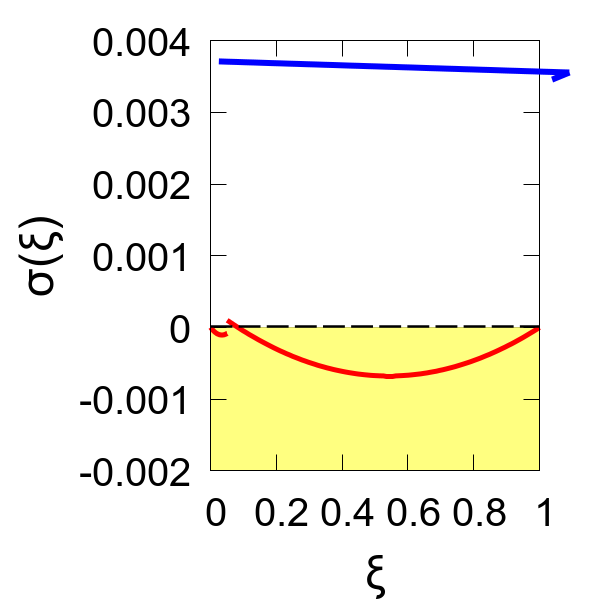
\includegraphics[width=1\textwidth]{plots/sigma_q_0.45_alpha_0.125pi.png}
		\end{minipage}
		\label{fig:10.c}
	}
	\\ 
	\subfigure[\tiny $q=0.35,\alpha=0.25\pi$]{
		\begin{minipage}[b]{0.25\textwidth}
			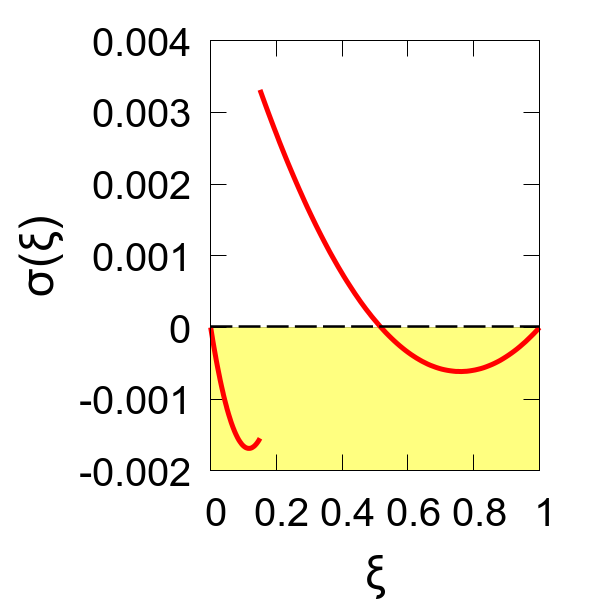
\includegraphics[width=1\textwidth]{plots/sigma_q_0.35_alpha_0.25pi.png} 
		\end{minipage}
		\label{fig:10.d}
	}
	\subfigure[\tiny $q=0.40,\alpha=0.25\pi$]{
		\begin{minipage}[b]{0.25\textwidth}
			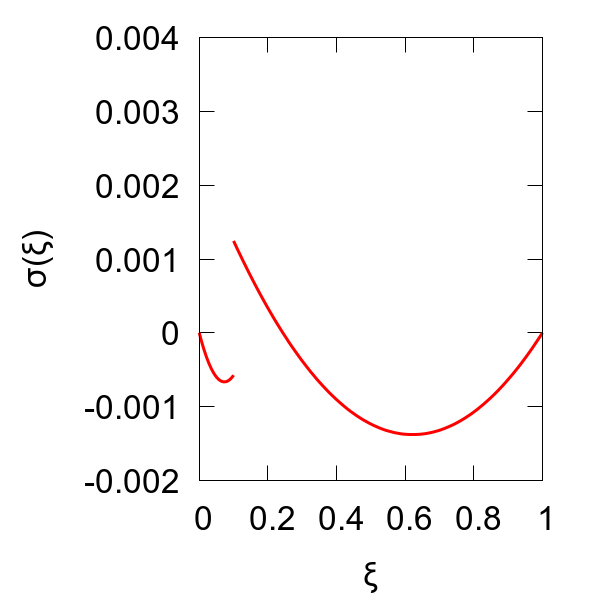
\includegraphics[width=1\textwidth]{plots/sigma_q_0.4_alpha_0.25pi.png}
		\end{minipage}
		\label{fig:10.e}
	}
	\subfigure[\tiny $q=0.45,\alpha=0.25\pi$]{
		\begin{minipage}[b]{0.25\textwidth}
			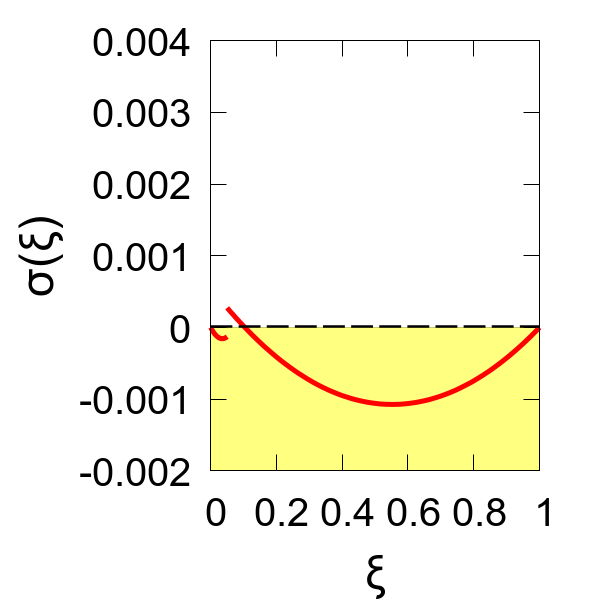
\includegraphics[width=1\textwidth]{plots/sigma_q_0.45_alpha_0.25pi.png}
		\end{minipage}
		\label{fig:10.f}
	}
\end{figure}
	\end{overlayarea}
\end{frame}

%%%%%%%%%%%%%%%%%%%%%%%%%%%%%%%%%%%%%%%%%%%%%%%%%%%%%%%%%%%%%%%%%%%%%%


\begin{frame}
	\frametitle{Summary}
	\begin{overlayarea}{\textwidth}{\textheight}
	\bi
	\item Consider the case of a single elastic particle in shear flow, as its motion is primarily governed by the background flow, not by interactions with other particles.
	\item Two of the four fixed orientations differ by an angle of $\pi$, but share the same shape.
	\item Initial configuration ($q,\alpha$) plays an important role in deformations.
	\item Four types of deformations observed.
	\item If the short arm is relative small, varying $\alpha$ may cause a bifurcation, creating a new closed loop in the steady orientation vs. FSI coefficient plot.
	\item No matter how complex the curve becomes, it always starts and ends at $\mathcal{I}=0$.
	\ei
	\end{overlayarea}
\end{frame}

%%%%%%%%%%%%%%%%%%%%%%%%%%%%%%%%%%%%%%%%%%%%%%%%%%%%%%%%%%%%%%%%%%%%%%
\begin{frame}
\begin{overlayarea}{\textwidth}{\textheight}
	\frametitle{Bibliography}
	\small
\bibliography{references}
\end{overlayarea}
\end{frame}
%%%%%%%%%%%%%%%%%%%%%%%%%%%%%%%%%%%%%%%%%%%%%%%%%%%%%%%%%%%%%%%%%%%%%%

\end{document}


